\documentclass[11pt, twoside]{book}
\usepackage[full]{leadsheets}
\usepackage[a4paper,  hmargin=1.5cm, vmargin=3cm, head=14pt, foot=50pt]{geometry}
\usepackage{multicol}
\usepackage[polish]{babel}
\usepackage{array}
\usepackage{graphicx}
\usepackage{hyperref}
\usepackage{tocloft}
\usepackage[toc]{multitoc}
\usepackage{fancyhdr}
\usepackage{tikzpagenodes}
\usepackage{titlesec}
\usepackage{tabularx}
\usepackage{adjustbox}
\usepackage{tipa}
\usepackage{ifxetex}
\usepackage[%
    left = \glqq,%
    right = \grqq,%
    leftsub = «,%
    rightsub = »%
]{dirtytalk}

\thispagestyle{empty}

\ifxetex%
    \usepackage{substitutefont}
    \substitutefont{T3}{\rmdefault}{cmr}
\fi

%\usepackage[default]{lato}
%\usepackage[T1]{fontenc}

\selectlanguage{polish}
\DeclareTranslation{Polish}{leadsheets/chorus}{Ref.}
\DeclareTranslation{Polish}{leadsheets/interlude}{Przej.}
\DeclareTranslation{Polish}{leadsheets/lyrics}{tekst}
\DeclareTranslation{Polish}{leadsheets/verse}{Zwr.}
%\DeclareTranslation{Polish}{leadsheets/capo}{Kapo}
\DeclareTranslation{Polish}{leadsheets/fret}{próg}

% Tytuł spisu treści
\addto\captionspolish{\renewcommand*\contentsname{Jakieś piosenki}}

\definesongproperty{annex}
\definesongtitletemplate{custom}{%
    \let\clearpage\relax
    \ifsongmeasuring%
        {\section*}
        {\section}%
        {\songproperty{title}}%
    \begingroup\footnotesize
        \begin{tabular}{%
                @{}
                >{\raggedright\arraybackslash}p{.5\linewidth}
                @{}
                >{\raggedleft\arraybackslash}p{.5\linewidth}
                @{}
            }
            \ifsongproperty{music}{%
                Muzyka: \songproperty{music}
                }{}%
            \ifsongproperty{annex}{%
                &
                \smash{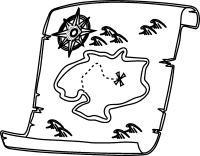
\includegraphics[height=40pt]{images/aneks-ref.png}}
                }{}%
            \ifsongproperty{music}{\\}{\ifsongproperty{annex}{\\}{}}%
            \ifsongproperty{lyrics}{%
                Tekst: \songproperty{lyrics} \\%
                }{}%
            \ifsongproperty{interpret}{%
                Interpretacja: \songproperty{interpret} \\%
                }{}%
            \ifsongproperty{capo}{%
                & \capo{} \\%
                }{}%
        \end{tabular}%
        \par
    \endgroup
}

\setleadsheets{%
    title-template = custom,
    verse/numbered,
    remember-chords=false,
    align-chords={l},
    capo-nr-format=arabic,
    bar-shortcuts
}
\setchords{%
    minor={lowercase},
    input-notation=german,
    output-notation=german
}

\renewcommand{\chaptermark}[1]{\markboth{#1}{}}

\fancypagestyle{plain}{%
    \fancyhf{}
    \fancyhead[L]{Jakieś piosenki}
    \fancyfoot[LE,RO]{\Large\thepage}
}
\fancypagestyle{szanty}{%
    \pagestyle{plain}
    \fancyhead[R]{Szanty}
    \fancyfoot[LO]{
\includegraphics[height=45pt]{images/kolo.png}}
    \fancyfoot[RE]{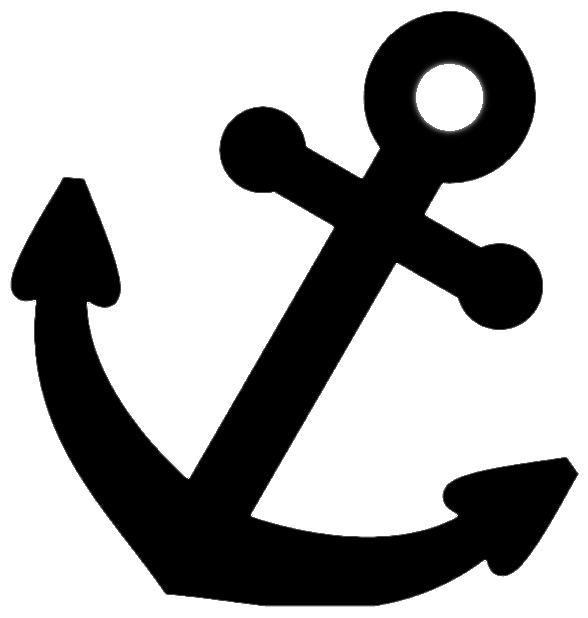
\includegraphics[height=45pt]{images/kotwica.png}}
}
\fancypagestyle{poezja}{%
    \pagestyle{plain}
    \fancyhead[R]{Poezja śpiewana}
    \fancyfoot[LO]{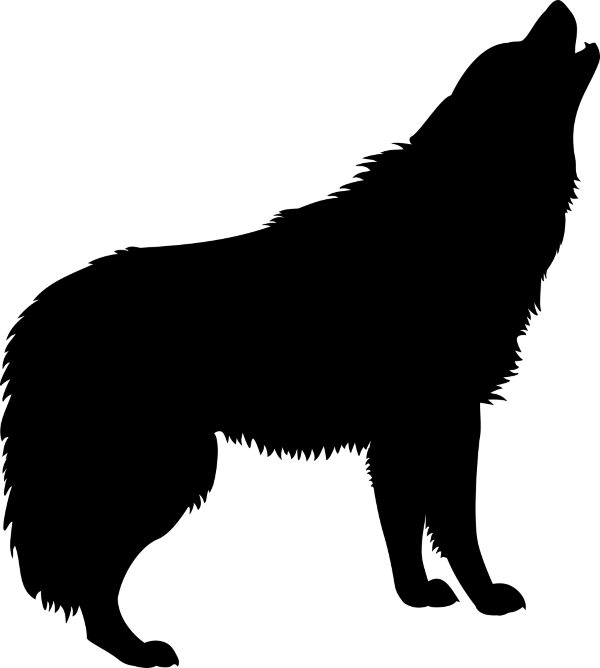
\includegraphics[height=45pt]{images/wilk.png}}
    \fancyfoot[RE]{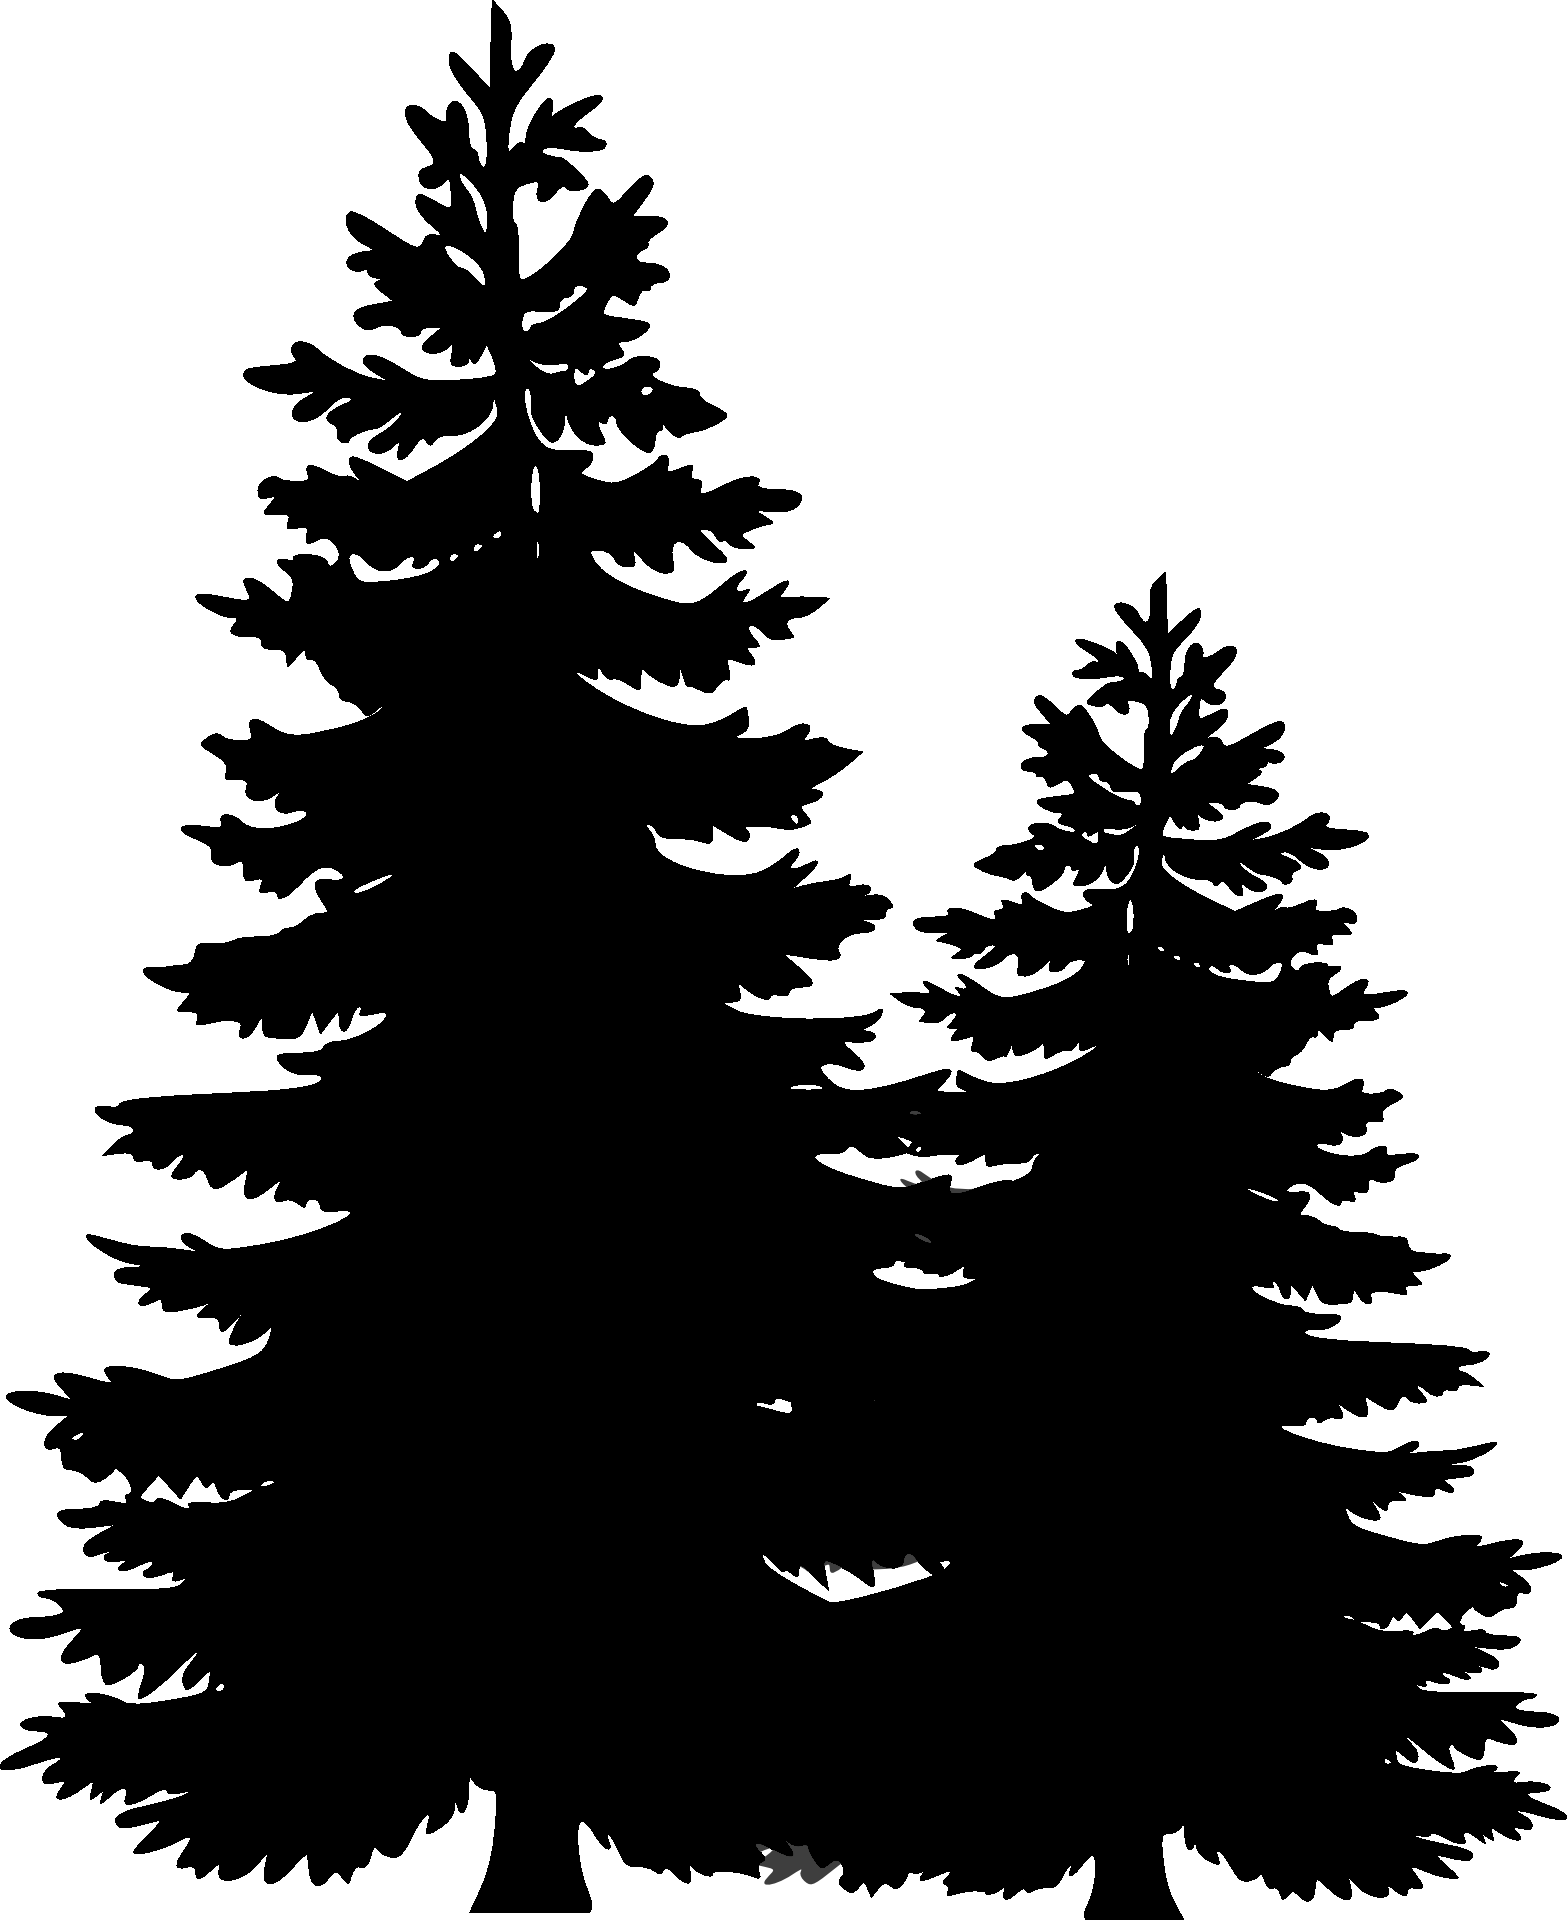
\includegraphics[height=45pt]{images/drzewa.png}}
}
\fancypagestyle{pop}{%
    \pagestyle{plain}
    \fancyhead[R]{Pop}
    \fancyfoot[LO]{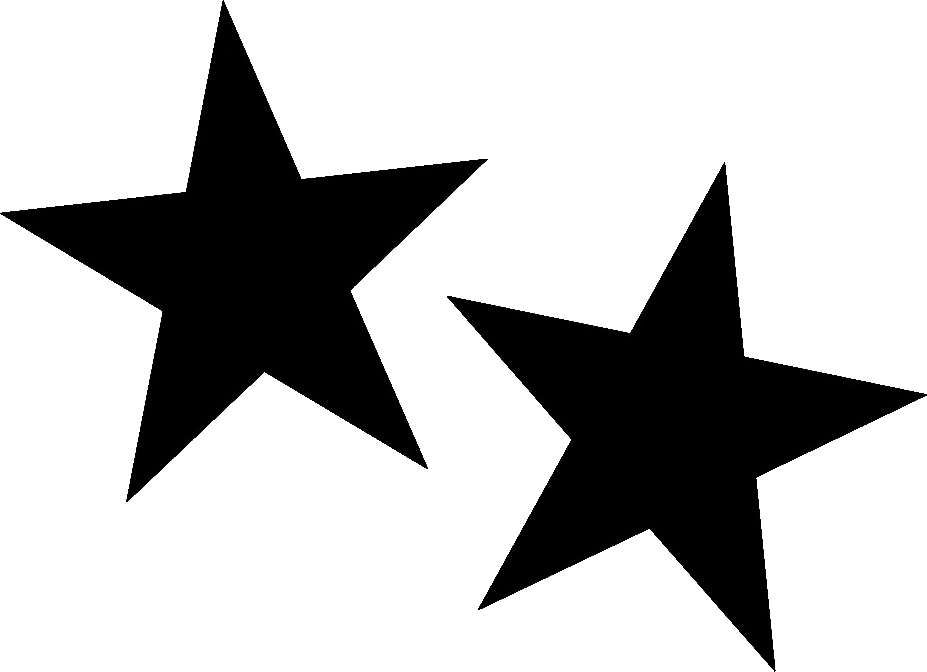
\includegraphics[height=45pt]{images/gwiazdy.png}}
    \fancyfoot[RE]{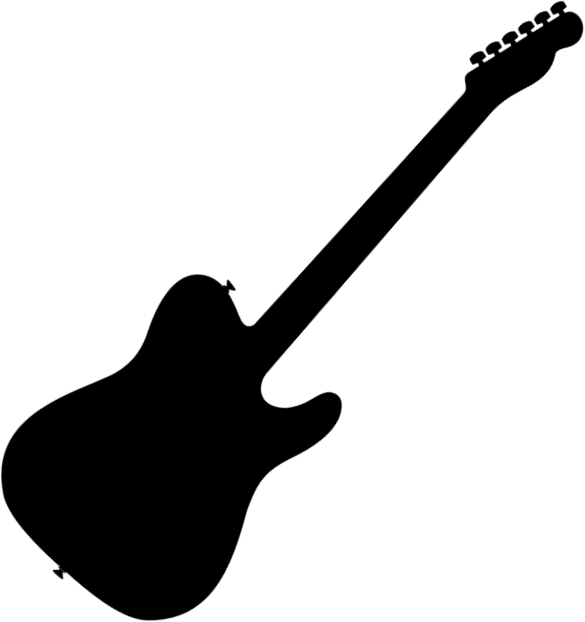
\includegraphics[height=45pt]{images/gitara.png}}
}

\renewcommand{\cftdot}{\ensuremath{\sim}}
\renewcommand{\cftsecleader}{\cftdotfill{\cftdotsep}}

% Usunięcie numeru rozdziału sprzed numeru sekcji
%\renewcommand{\thesection}{\arabic{section}}

\titleformat{\chapter}[block]{\centering\vspace{6cm}}{}{0pt}{\Huge\bfseries}

\newversetype{riff}[name={Riff}, numbered=false, named=true]

\counterwithin*{footnote}{section}


\begin{document}

\begin{titlepage}
    \begin{center}
        \vspace*{5cm}
        
        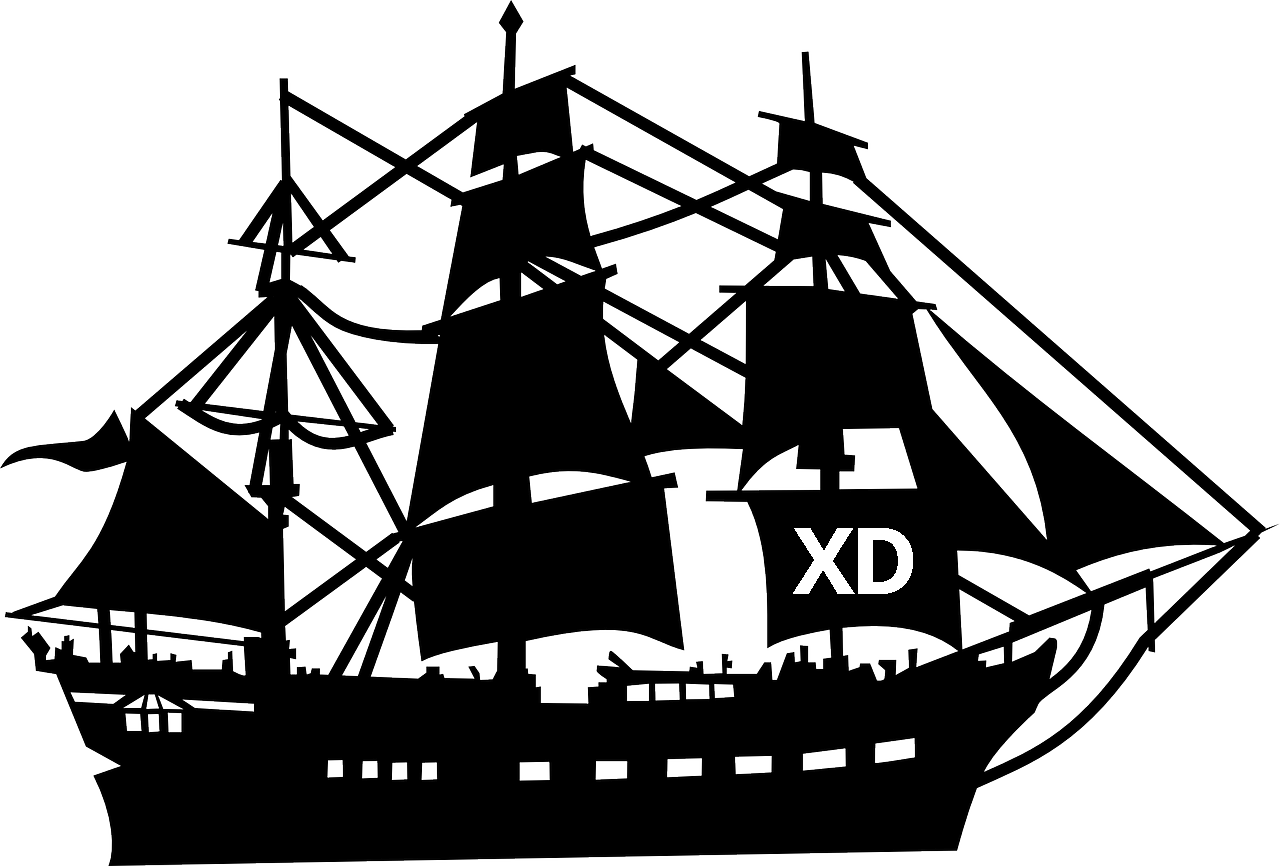
\includegraphics[height=8cm]{images/front-obrazek.png}

        \vspace{1.5cm}

        \Huge\textbf{Jakieś piosenki}
        
        \vspace{0.5cm}
        
        \LARGE Wydanie pierwsze
        
        \vfill

        \Large
        Wydawnictwo Kis Inkris \\
        Warszawa, 2021

        %\vspace{0.5cm}

        %\footnotesize
        %https://github.com/dzierzanowski/spiewnik-szant

        %\begin{tikzpicture}[remember picture,overlay,shift={(current page.south east)}]
        %    \node[anchor=south east,xshift=0cm,yshift=0cm]{
\includegraphics[width=3.5cm]{images/qr.png}};
        %\end{tikzpicture}
    \end{center}
\end{titlepage}

\tableofcontents
\vfill
\renewcommand{\tabularxcolumn}[1]{>{\small}b{#1}}
\begin{adjustbox}{width={\textwidth}, keepaspectratio}
\begin{tabularx}{\textwidth}{%
        @{}
        >{\raggedright\arraybackslash}X
        @{}
        >{\raggedleft\arraybackslash}X
    }
    \footnotesize
    Kamil Dzierżanowski --- opracowanie, skład, korekta

    Paweł Kulig --- opracowanie

    \medskip

    Daj śpiewnikowi gwiazdkę na GitHubie:

    \smallskip

    \urlstyle{same}
    \url{https://github.com/dzierzanowski/spiewnik-szant}

    &

    Pobierz śpiewnik online:

    \smallskip

    
\includegraphics[width=3cm]{images/qr.png}
\end{tabularx}
\end{adjustbox}


\chapter{Szanty}
\begin{center}
    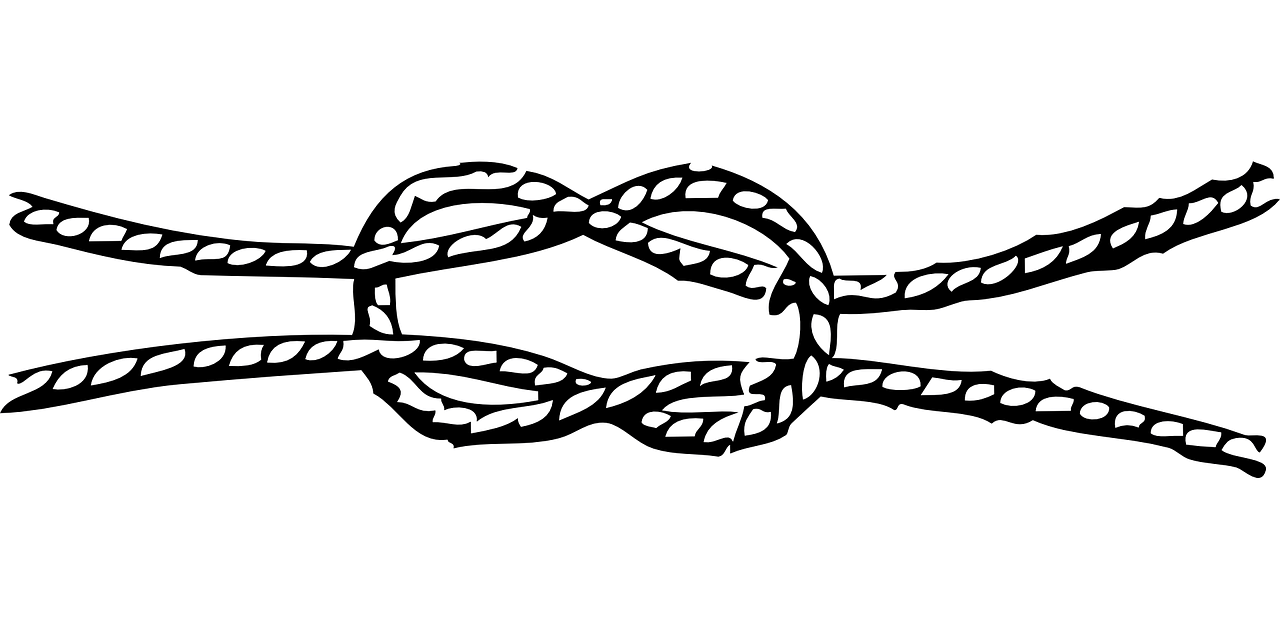
\includegraphics[width=0.5\textwidth]{images/wezel.png}
\end{center}
\pagestyle{szanty}
\newpage
\begin{song}{title={Bitwa}, music={Mechanicy Shanty}}
\begin{multicols}{2}
    \begin{intro}
        e h C a \\
        e D e e
    \end{intro}
    \begin{verse}
        ^{e}Okręt nasz w^{h}płynął w mgłę ^{C}i fregaty d^{a}wie \\
        Popłyn^{e}ęły ^{D}naszym kursem ^{G}by nie zgubić s^{H7}ię \\
        ^{e}Potem szkwał w^{h}ypchnął nas ^{C}poza mleczny ^{a}pas \\
        I nikt wt^{e}edy n^{D}ie przypuszczał, ^{G}że fregaty ^{H7}śmierć nam niosą
    \end{verse}
    \begin{chorus}
        ^{G}Ciepła kr^{D}ew poleje ^{e}się strug^{h}ami \\ 
        ^{C}Wygra ten, k^{a}to utrz^{D}yma ^{e}ship \\
        W ^{G}huku dział ^{D}ktoś przykryje ^{e}się fal^{h}ami \\
        ^{C}Jak da Bóg, ^*{a}ocal ^{D}imy ^{e}bryg
    \end{chorus}
    \begin{verse}
        Nagły huk w uszach grał i już atak trwał \\
        To fregaty uzbrojone rzędem w setkę dział \\
        Czarny dym spowił nas, przyszedł śmierci czas \\
        Krzyk i lament mych kamratów, przerywany ogniem katów
    \end{verse}
    \begin{chorus}
        Ciepła krew poleje się strugami\ldots
    \end{chorus}
    \begin{verse}
        Pocisk nasz trafił w maszt, usłyszałem trzask \\
        To sterburtę rozwaliła jedna z naszych salw \\
        "Żagiel staw" krzyknął ktoś, znów piratów złość \\
        Bo od rufy nam powiało, a fregatom w mordę wiało
    \end{verse}
    \begin{chorus}
        Ciepła krew poleje się strugami\ldots
    \end{chorus}
    \begin{verse}
        Z fregat dwóch tylko ta pierwsza w pogoń szła \\
        Wnet abordaż rozpoczęli, gdy dopadli nas \\
        Szyper ich dziury dwie zrobił w swoim dnie \\
        Nie pomogło to psubratom, reszta z rei zwisa za to
    \end{verse}
    \begin{chorus}
        Ciepła krew poleje się strugami\ldots
    \end{chorus}
    \begin{verse}
        Po dziś dzień tamtą mgłę i fregaty dwie \\
        Kiedy noc zamyka oczy, widzę w moim śnie \\
        Tamci, co śpią na dnie, uśmiechają się \\
        Że ich straszną śmierć pomścili bracia, którzy zwyciężyli
    \end{verse}
    \begin{chorus}
        Ciepła krew poleje się strugami\ldots
    \end{chorus}
\end{multicols}
\end{song}


\newpage
\begin{song}{title={Chłopcy z Botany Bay}, music={Mietek Folk}, capo=3}
\begin{multicols}{2}
    \begin{verse}
        Już nad ^{h}Hornem ^{A}zapada ^{h}noc ^{h} \\
        Wiatr na ^{h}żaglach ^{A}położył ^{D}się ^{D} \\
        |: A tam ^{G}jeszcze ^{A}korsarze na ^*{D}Bota ^{A}ny ^{h}Bay | \\
        | Upy^{G}chają ^{A}zdobycze ^{h}swe :|
    \end{verse}
    \begin{verse}
        Jolly Roger na maszcie już śpi \\
        Jutro przyjdzie z Hiszpanem się bić \\
        A korsarze znużeni na Botany Bay \\
        Za zwycięstwo dziś będa swe pić
    \end{verse}
    \begin{verse}
        Śniady Clark puchar wznosi do ust \\
        "Bracia, toast! Niech idzie na dno!" \\
        Tylko Johnny nie pije, bo kilka mil stąd \\
        Otuliło złe morze go
    \end{verse}
    \begin{verse}
        Nie podnosi kielicha do ust \\
        Zawsze on tu najgłośniej się śmiał \\
        Mistrz fechtunku z Florencji ugodził go \\
        Już nie będzie za szoty się brał
    \end{verse}
    \begin{verse}
        W starym porcie zapłacze Margot \\
        Jej kochany nie wróci już \\
        Za dezercję do panny na kei w Brisbane \\
        Oddać musiał swą głowę pod nóż
    \end{verse}
    \begin{verse}
        Tak niewielu zostało dziś ich \\
        Resztę zabrał Neptun pod dach \\
        Choć na ustach wciąż uśmiech, to w sercach lód \\
        W kuflu miesza się rum i strach
    \end{verse}
    \begin{verse}
        To ostatni chyba już rejs \\
        Cios sztyletem lub kula w pierś \\
        Bóg na szkuner w niebiosach zabierze ich \\
        Wszystkich chłopców z Botany Bay
    \end{verse}
    \begin{verse}
        Już nad Hornem zapada noc \\
        Wiatr na żaglach położył się \\
        A tam jeszcze korsarze na Botany Bay \\
        Upychają zdobycze swe
    \end{verse}
\end{multicols}
\end{song}


\newpage
\begin{song}{title={Dziesięć w skali Beauforta}, music={Krzysztof Klenczon}, capo=3, annex}
    \begin{multicols}{2}
    \begin{verse}
        Ko^{e}łysał nas zac^{a}hodni wiatr \\
        ^{H7}Brzeg gdzieś za rufą z^{e}ostał \\
        I n^{a}agle ktoś jak p^{e}apier zbladł \\
        ^{F#7}Sztorm idzie, panie ^{H}bosman
    \end{verse}
    \begin{chorus}
        A ^*{C}bo sm^{G}an tylko ^{C}zapiął pł^{G}aszcz \\
        I z^{C}aklął: \say{^{H7}Ech, do cz^{e}orta \\
        Nie da^{C}ję ła^{D}jbie ż^{G}adnych s^{e}zans} \\
        ^{e}Dziesięć w ^{a}skali ^*{H7}Beau ^{e}forta
    \end{chorus}
    \vfill\null\columnbreak{}
    \begin{verse}
        Z zasłony ołowianych chmur \\
        Ulewa spadła nagle \\
        Rzucało nami w górę, w dół \\
        I fala zmyła żagle
    \end{verse}
    \begin{chorus}
        A bosman tylko zapiął płaszcz\ldots
    \end{chorus}
    \begin{verse}
        Gdzie został ciepły, cichy kąt \\
        I brzegu kształt znajomy \\
        Zasnuły mgły daleki ląd \\
        Dokładnie, z każdej strony
    \end{verse}
    \begin{chorus}
        A bosman tylko zapiął płaszcz\ldots
    \end{chorus}
    \begin{verse}
        O pokład znów uderzył deszcz \\
        I padał już do rana \\
        Piekielnie ciężki to był rejs \\
        Szczególnie dla bosmana
    \end{verse}
    \begin{chorus}
        A bosman tylko zapiął płaszcz \\
        I zaklął: \say{Ech, do czorta \\
        Przedziwne czasem sny się ma} \\
        Dziesięć w skali Beauforta \medskip \\
        Dziesięć w skali Beauforta \\
        Dziesięć w skali Beauforta
    \end{chorus}
    \end{multicols}
\end{song}


\newpage
\begin{song}{title={Few days}, music={Ryczące Dwudziestki}, annex}
\begin{multicols}{2}
    \begin{verse}
        O Panie, czemu w ziemi tkwię \\
        Hej raz, hej raz! \\
        I macham szuflą cały dzień? \\
        Hej, na morze czas!
    \end{verse}
    \begin{chorus}
        Mogę kopać tu dalej \\
        Few days, few days \\
        Mogę kopać przez dni parę \\
        Ale wracać chcę $\times 2$
    \end{chorus}
    \begin{verse}
        Tam każdy takie bajdy plótł \\
        Nie raz, nie raz \\
        Przekroczysz Jukon, złota w bród \\
        Hej, na morze czas!
    \end{verse}
    \begin{chorus}
        Mogę kopać tu dalej\ldots $\times 2$ 
    \end{chorus}
    \vfill\null\columnbreak{}
    \begin{verse}
        Wykopię jeszcze parę dziur \\
        Hej raz, hej raz \\
        Wytoczę płonnej skały wór \\
        Hej, na morze czas!
    \end{verse}
    \begin{chorus}
        Mogę kopać tu dalej\ldots $\times 2$ 
    \end{chorus}
    \begin{verse}
        Za żonę tu łopatę mam \\
        Już dość, już dość \\
        A zysk, że jej uzywam sam \\
        Hej, na morze czas!
    \end{verse}
    \begin{chorus}
        Mogę kopać tu dalej\ldots $\times 2$
    \end{chorus}
    \begin{verse}
        O Panie nie jest to Twój raj \\
        O nie, o nie \\
        Nadzieję innym głupcom daj \\
        Ja na morze chcę!
    \end{verse}
    \begin{chorus}
        Chociaż już mi wystarczy \\
        Few days, few days \\
        Dam Ci jeszcze jedną szansę \\
        Ale wracać chcę $\times 2$
    \end{chorus}
\end{multicols}
\end{song}


\newpage
\begin{song}{title={Gdzie ta keja}, music={Jerzy Porębski}, interpret={Trzy Majtki}}
    \begin{verse}
        Gdyby ^{a}tak ktoś przyszedł i powiedział: \say{S^{E}tary, czy masz ^{a}czas? \\
        Potrze^{C}buję do załogi j^{G}akąś nową t^{C}warz \\
        Ama^{C}zonka, Wielka R^{C7}afa, ^{d} oceany trzy \\
        Rejs na ^{a}całość, rok, dwa lata} --- ^{E}to powiedział^{a}bym:
    \end{verse}
  	\begin{chorus}
        Gdzie ta ^{a}keja, a ^{E}przy niej ten j^{a}acht \\
        Gdzie ta ^{C}koja, ^{G}wymarzona w s^{C}nach \\
        Gdzie te w^{g}szystkie sz^{A7}nurki ^{d}od ^{A7}tych sz^{d}mat \\
        Gdzie ta b^{a}rama ^{E}na szeroki ś^{a}wiat
    \end{chorus}
    \begin{chorus*}
        Gdzie ta keja, a przy niej ten jacht \\
        Gdzie ta koja wymarzona w snach \\
        W każdej chwili płynę w taki rejs \\
        Tylko gdzie to jest, no gdzie to jest
    \end{chorus*}
    \begin{verse}
        Gdzieś na dnie wielkiej szafy leży ostry nóż \\
        Stare jeansy wystrzępione impregnuje kurz \\
        W kompasie igła zardzewiała, lecz kierunek znam \\
        Biorę wór na plecy i przed siebie gnam
    \end{verse}
  	\begin{chorus}
        Gdzie ta keja, a przy niej ten jacht\ldots
    \end{chorus}
    \begin{verse}
        Przeszły lata zapyziałe, rzęsą zarósł staw \\
        A na przystani czółno stało --- kolorowy paw \\
        Zaokrągliły się marzenia, wyjałowiał step \\
        Lecz dalej marzy o załodze ten samotny łeb
    \end{verse}
  	\begin{chorus}
        Gdzie ta keja, a przy niej ten jacht\ldots
    \end{chorus}
\end{song}


\newpage
\fancyfoot[LO,RE]{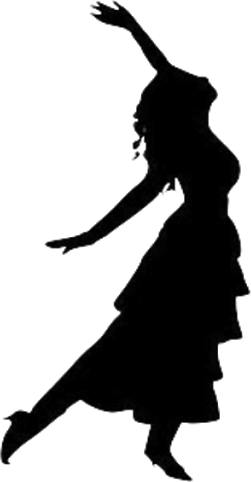
\includegraphics[height=45pt]{images/hiszpanska-dziewczyna.png}}
\begin{song}{title={Hiszpańskie dziewczyny}, music={tradycyjna angielska (Spanish Ladies)}, lyrics={Ryczące Dwudziestki}, capo={2}, annex}
    \begin{intro}
        Żegnajcie nam dziś, hiszpańskie dziewczyny \\
        Żegnajcie nam dziś, marzenia ze snów \\
        Ku brzegom angielskim już rzuszać nam pora \\
        Lecz kiedyś na pewno wró^{F#7}cimy tu z^{h}nów
    \end{intro}
    \begin{chorus}
        I s^{h}mak waszych ust, hiszpańskie dziew^{f#}czyny \\
        W noc ^{h}ciemną i złą nam będzie się ^{A}śnił \\
        Le^{G}niwie pop^{A}łyną znów ^{D}rejsu go^{h}dziny \\
        Wspom^{G}nienie ust waszych przys^{F#7}porzy nam ^{h}sił $\times 2$
    \end{chorus}
    \begin{verse}
        Nie^{h}długo ujrzymy znów w dali Cape ^*{f#}Dead man\footnotemark{} \\
        I Gł^{h}owę Baranią\footnotemark{} sterczącą wśród wz^{A}górz \\
        I s^{G}tatki sto^{A}jące na ^{D}redzie przed ^{h}Plymouth \\
        Kla^{G}rować kotwicę naj^{F#7}wyższy czas ^{h}już
    \end{verse}
    \begin{chorus}
        I smak waszych ust, hiszpańskie dziewczyny\ldots $\times 2$
    \end{chorus}
    \begin{verse}
        I znów białe żagle na masztach rozkwitną \\
        Kurs szyper wyznaczy do Portland i Wight\footnotemark{} \\
        I znów stara łajba potoczy się ciężko \\
        Przez fale, w kierunku na Beachy, Fairlight\footnotemark{}
    \end{verse}
    \begin{chorus}
        I smak waszych ust, hiszpańskie dziewczyny\ldots $\times 2$
    \end{chorus}
    \begin{verse}
        Zabłysną nam bielą skał zęby pod Dover \\
        I znów noc w kubryku wśród legend i bajd \\
        Powoli i znojnie tak płynie nam życie \\
        Na wodach i w portach South Foreland Light\footnotemark{}
    \end{verse}
    \begin{chorus}
        I smak waszych ust, hiszpańskie dziewczyny\ldots $\times 2$
    \end{chorus}
    \footnotetext{Dodman Point, Kornwalia; nie mylić z Cape Diamond, Quebec City --- to po innej stronie oceanu}
    \footnotetext{Ram Head, Kornwalia}
    \footnotetext{Isle of Wight (\textipa{/waIt/})}
    \footnotetext{Beachy Head i Fairlight, East Sussex}
    \footnotetext{wiktoriańska latarnia morska w South Foreland, Kent; nie ustalono, co autor miał na myśli}
\end{song}

\newpage\pagestyle{szanty}
\newpage
\begin{song}{title={Jasnowłosa}, lyrics={Ryczące Dwudziestki}}
    \begin{verse}
        Na ^{G}tańcach ją poznałem, długo^*{C}wło ^{D}są ^{G}blond \\
        Dziew^{G}czynę moich ^{e}marzeń, nie wia^{C}domo ^{D}skąd \\
        ^{G}Ona się tam ^{e}wzięła, piękna ^{C}niczym ^*{F}kwia ^{D7}t \\
        Czy jak sy^{G}rena wyszła z morza, czy ją ^*{C}przy ^{D}gnał ^{G}wiatr?
    \end{verse}
    \begin{chorus}
        ^{G}Żegnaj, Irlandio, czas w ^{C}drogę ^{D} mi ^{G}już \\
        W ^{G}porcie go^{e}towa stoi ^{C}moja ^{D}łódź \\
        Na ^{G}wielki o^{e}cean przyjdzie ^{C}mi zaraz ^*{F}wy ^{D7}jść \\
        I po^{G}żegnać się z dziewczyną na ^*{C}Loughin ^*{D}sho ^{G}lin
    \end{chorus}
    \begin{verse}
        Ująłem ją za rękę delikatną, jak \\
        Latem mały motyl albo róży kwiat \\
        Poszedłem z nią na plażę, wsłuchać się w szum fal \\
        Pokazałem jasnowłosej wielki morza czar
    \end{verse}
    \begin{chorus}
        Żegnaj, Irlandio, czas w drogę mi już\ldots
    \end{chorus}
    \begin{verse}
        Za moment wypływam w długi, trudy rejs \\
        I z piękną mą dziewczyną przyjdzie rozstać się \\
        Żagle pójdą w górę, wiatr mnie pogna w przód \\
        I przez morza mnie powiedzie, ty zostaniesz tu
    \end{verse}
    \begin{chorus}
        Żegnaj, Irlandio, czas w drogę mi już\ldots $\times 2$
    \end{chorus}
\end{song}


\newpage
\begin{song}{title={Kapitan Kidd}, music={North Cape}}
\begin{multicols}{2}
    \begin{chorus}
        Me ^{e}imię ^{h}William ^{e}Kidd \\
        Już czeka ^{a}stryk, czeka ^{D}stryk \\
        Królewski ^{e}korsarz ^{h}William ^{e}Kidd, czeka ^*{G}stry ^{D}k \\
        Me ^{G}imię ^{D}William ^{a}Kidd \\
        Zbrodni ^*{e}ogrom ^{h}nych to ^{a}mit \\
        Powró^{e}ciłem, ^{G}choć w Lon^{h}dynie ^{D/F#}czeka ^{e}stryk
    \end{chorus}
    \begin{verse}
        Mój ^{e}ojciec ^{h}uczył ^{e}mnie \\
        Jak nie ^{G}znaleźć się na ^{D}dnie \\
        Lecz los o^{e}krutny ^{D}zabrał ^{a}go ro^{h}dzinie ^{e}mej \\
        Choć biblię w ^{e}rękę ^{h}moją ^{e}kładł \\
        Morza ^{G}urok na mnie ^{D}padł \\
        I mary^{e}narzem ^{D}stałem ^{a}się, choć ^{h}czeka ^{e}stryk
    \end{verse}
    \begin{chorus}
        Me imię William Kidd\ldots
    \end{chorus}
    \begin{verse}
        Kanonier William Moore \\
        Pierwszy trafił na mój sznur \\
        Bo przeciw mnie ośmielił się on wzniecić bunt \\
        Choć dobrym strzelcem William był \\
        Pod salingiem będzie gnił \\
        Buntownik każdy skończy tak, już czeka stryk
    \end{verse}
    \begin{chorus}
        Me imię William Kidd\ldots
    \end{chorus}
    \begin{verse}
        Raz gdy było ze mną źle \\
        Obiecałem sobie, że \\
        Mądrości drogą odtąd pójdę po kres dni \\
        Lecz mój korsarski podły fach \\
        Zabił wnet o duszę strach \\
        I potępienie czeka mnie, bo czeka stryk
    \end{verse}
    \begin{chorus}
        Me imię William Kidd\ldots
    \end{chorus}
    \begin{verse}
        \textit{(wolniej)} \\
        To egzekucyjny blok \\
        Zaraz mnie ogarnie mrok \\
        Bo na mą szyję kat założy gruby sznur \\
        Więc dzisiaj ostrzec ciebie chcę \\
        Byś za przykład nie brał mnie \\
        Mądrości drogą zawsze szedł, bo czeka stryk
    \end{verse}
    \begin{chorus}
        \textit{(szybciej)} \\
        Me imię William Kidd\ldots
    \end{chorus}
\end{multicols}
\end{song}
\newpage

\newpage
\begin{song}{title={Morze, moje morze}, music={EKT Gdynia}}
    \begin{intro}
        \writechord{d} \writechord{g} \writechord{F} \writechord{A7} \\
        \writechord{d} \writechord{g} \writechord{A7} \writechord{d}
    \end{intro}
    \begin{multicols}{2}
    \begin{verse}
        ^{d}Hej, me Bał^{A7}tyckie Mo^{d}rze ^{C} \\
        W^{F}dzięczny ci ^{C}jestem bar^{F}dzo \\
        |: ^{g}Toś ty mnie ^{C}wychowało \\
        ^{F} Toś ty mnie ^{g}wychowało \\
        Sz^{d}kołęś mi ^{A}dało twar^{d}dą :|
    \end{verse}
    \begin{verse}
        Szkołęś mi dało twardą \\
        Uczyłoś łodzą pływać \\
        Żagle pięknie cerować, \\
        Żagle pięknie cerować, \\
        Codziennie pokład zmywać
    \end{verse}
    \begin{verse}
        Codziennie pokład zmywać \\
        Od soli i od kurzy \\
        Mosiądze wyglansować \\
        Mosiądze wyglansować \\
        W ciszy, czy w czasie burzy
    \end{verse}
    \begin{center}
        \vspace{0.6cm}
        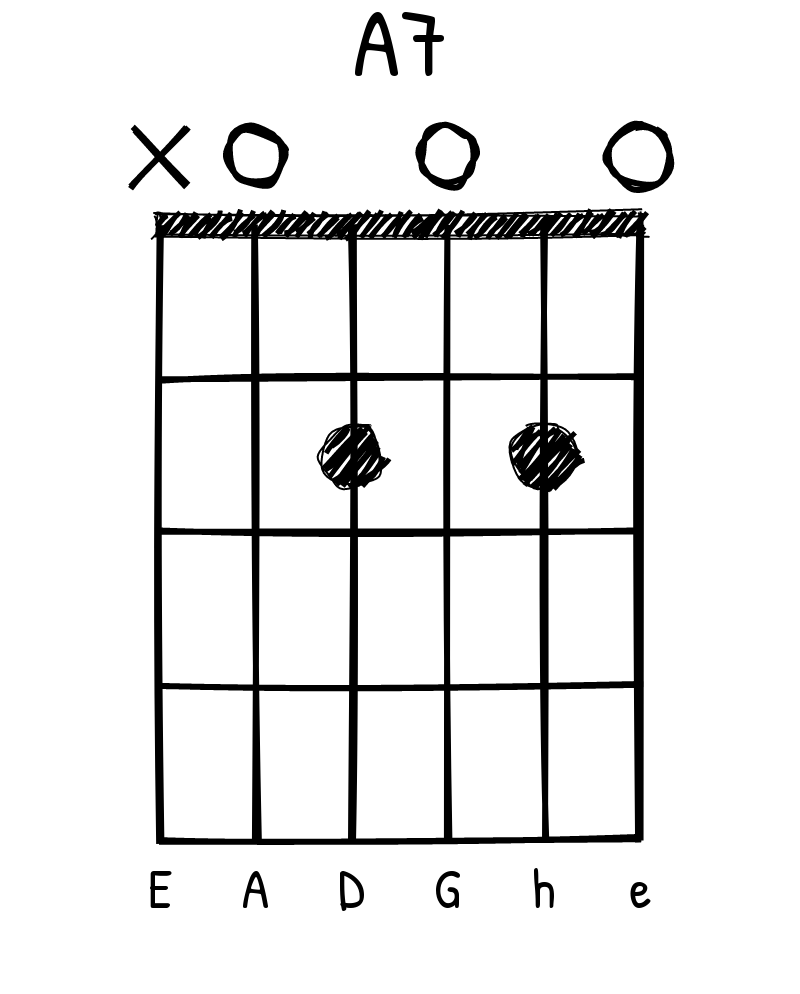
\includegraphics[height=3.5cm]{images/A7.png}
    \end{center}
    \vfill\null\columnbreak{}
    \begin{verse}
        W ciszy, czy w czasie burzy \\
        Trzeba przy pracy śpiewać \\
        Bo kiedy śpiewu nie ma \\
        Bo kiedy śpiewu nie ma \\
        Neptun się będzie gniewać
    \end{verse}
    \begin{verse}
        Neptun się będzie gniewać \\
        I klątwę brzydką rzuci \\
        Wpakuje na mieliznę \\
        Wpakuje na mieliznę \\
        Albo nam łódź wywróci
    \end{verse}
    \begin{verse}
        Albo nam łódź wywróci \\
        I krzyknie: \say{Hej, partacze! \\
        Nakarmię wami rybki \\
        Nakarmię wami rybki \\
        Nikt po was nie zapłacze!}
    \end{verse}
    \begin{verse}
        Nikt po nas nie zapłacze \\
        Nikt nam nie dopomoże \\
        Za wszystkie miłe rady \\
        Za wszystkie miłe rady \\
        Dziękuję tobie, Morze
    \end{verse}
    \begin{verse}
        Hej, Morze, moje Morze \\
        Wdzięczny ci jestem bardzo \\
        Toś ty mnie wychowało \\
        Toś ty mnie wychowało \\
        Szkołęś mi dało twardą
    \end{verse}
    \end{multicols}
\end{song}


\newpage
\begin{song}{title={Nazywali go Marynarz (Szanta narciarska)}, music={Artur Andrus}}
	\begin{intro}
	\writechord{d}
	\end{intro}    
    \begin{multicols}{2}
    \begin{verse}
        Nazy^{d}wali ^{C}go ma^{d}rynarz \\
        Bo o^{d}paskę ^{C}miał na ^{d}oku \\
        ^{g}Na każdym stoku dziew^{d}czyna \\
        Dziew^{B}czyna na ^{A}każdym s^{d}toku
    \end{verse}
    \begin{verse*}
        Po^{d}chodzi s^{C}pod Poz^{d}nania \\
        Po^{d}dobno ^{C}umie w^{F}różyć z kart \\
        ^{g}Panny rwie na wią^{d}zania \\
        Mę^{B}żatki --- ^{A}na długość ^{d}nart
    \end{verse*}
  	\begin{chorus}
        Ca^{d}ryco ^{A}mokrego ś^{d}niegu \\
        Ra^{d}trakiem płynę do ciebie pod ^{g}prąd --- hej! \\
        ^{g}Dobrze, że stoisz na ^{d}brzegu \\
        Bo ja ^{B}właśnie ^{A}schodzę na ^{d}ląd
    \end{chorus}
        \vfill\null\columnbreak{}
    \begin{verse}
        Nigdy się nie lękał biedy \\
        I się nie przejmował jutrem \\
        A jego ratrak był kiedyś \\
        Zwyczajnym, rybackim kutrem
    \end{verse}
    \begin{verse*}
        I woził dorsze i śledzie \\
        Zimą i latem, okrągły rok \\
        Teraz, jak nieraz przejedzie \\
        Rybami --- czuć cały stok
    \end{verse*}
    \begin{chorus}
        Caryco mokrego śniegu\ldots
    \end{chorus}
    \begin{verse}
        Wszyscy w porcie odetchnęli \\
        Zwiał, nim się zakończył sezon \\
        Jeszcze się tam, jak żagiel bieli \\
        Jego czarny kombinezon
    \end{verse}
    \begin{verse*}
        Odpłynął pod Ustrzyki \\
        I przez kobiety wpadł w kłopoty \\
        Forsę z polowań na orczyki \\
        Przehulał --- na antybiotyk
    \end{verse*}
    \begin{chorus}
        Caryco mokrego śniegu\ldots
    \end{chorus}
    \begin{verse}
        Jeśli kiedyś go zobaczysz \\
        Na ratraku w podłym świecie \\
        To powiedz mu, że w Karpaczu \\
        Czekają na niego dzieci
    \end{verse}
    \begin{verse*}
        I kiedy opuszcza statek \\
        Żeby się znowu oddać złu \\
        Każda z dwudziestu siedmiu matek \\
        Dzieciątku --- śpiewa do snu
    \end{verse*}
    \begin{chorus}
        Caryco mokrego śniegu\ldots $\times 2$
    \end{chorus}
    \end{multicols}
\end{song}


\newpage
\begin{song}{title={Pieśń wielorybników}, interpret={EKT Gdynia}, music={tradycyjna (Bonnie Ship the Diamond)}}
\begin{multicols}{2}
    \begin{intro}
        a a a d \\
        a e a a $\times 2$
    \end{intro}
    \begin{verse}
        Nasz D^{a}iament prawie g^{e}otów już \\
        W cieśn^{a}inach nie ma kr^{e}y \\
        Na k^{a}ei piękne pa^{e}nny stoją \\
        W ich o^{d}czach bły^{e}szczą ł^{a}zy \\
        Kapitan w niebo wlepia wzrok \\
        Ruszamy lada dzień \\
        Płyniemy tam, gdzie słońca blask \\
        nie mąci nocy cień
    \end{verse}
    \begin{chorus}
        A więc krz^{a}ycz: ^{e}o h^{a}o! \\
        Odw^{a}agę w s^{e}ercu mi^{a}ej \\
        Wielor^{a}ybów ci^{e}elska gr^{C}oźne s^{G}ą \\
        Lecz do^*{F}sta ni^{e}emy j^{a}e $\times 2$
    \end{chorus}
    \begin{chorus*}
        a a a d \\
        a e a a $\times 2$
    \end{chorus*}
    \begin{verse}
        Ej panno powiedz po co łzy \\
        Nic nie zatrzyma mnie \\
        Bo prędzej w wodach kwiat zakwitnie \\
        Niż wycofam się \\
        No nie płacz mała, wrócę tu \\
        Nasz los nie taki zły \\
        Bo da dukatów wór za tran \\
        I wielorybie kły
    \end{verse}
    \begin{chorus}
        A więc krzycz: o ho!\ldots $\times 2$
    \end{chorus}
    \begin{verse}
        Na deku stary wąchał wiatr \\
        lunetę w ręku miał \\
        Na łodziach co zwisały już \\
        z harpunem każdy stał \\
        I dmucha tu i dmucha tam  \\
        ogromne stado w krąg \\
        Harpuny, wiosła, liny brać \\
        I ciągnij brachu ciąg
    \end{verse}
    \begin{chorus}
        A więc krzycz: o ho!\ldots $\times 2$
    \end{chorus}
    \begin{verse}
        \textit{wolniej} \\
        I dla ^*{a}wielo ry^{G}ba j^{a}uż \\
        Os^*{e}ta tn^{G}i to dzi^{a}eń \\
        Bo śmi^{a}ały harp^*{C}u nn^{G}ik \\
        ^*{F}U de^{G}rza w^{a}eń
    \end{verse}
    \begin{outro}
        a a a d \\
        a e a a
    \end{outro}
\end{multicols}
\end{song}
\fancyfoot[LO,RE]{
\includegraphics[height=45pt]{images/docker.png}}

\newpage\pagestyle{szanty}
\newpage
\begin{song}{title={Pij za starego (Whiskey in the jar)}, music={Thin Lizzy}, interpret={Poszedłem Na Dziób}}
    \begin{intro}
        \writechord{F} \writechord{C} \writechord{G} \writechord{C}
    \end{intro}
    \begin{multicols}{2}
    \begin{verse}
        Pły^{C}nąłem w dół Cork City \\
        By ^{a}przejść przez Góry Kerry \\
        Spot^{F}kałem tam Farrella \\
        Co ^{C}forsę swoją liczył \\
        Sięg^{C}nąłem więc po spluwę \\
        A ^{a}potem po swój rapier \\
        Krzyk^{F}nąłem: \say{Dawaj forsę \\
        Jeśli ^{C}ci miłe życie!}
    \end{verse}
    \begin{chorus}
        $\times 2$ \\
        Masza ^{G}ring dama du dama da \\
        ^{C} Pij za starego \\
        ^{F} Pij za starego \\
        Bo ^{C}whiskey ^{G}pełny ^{C}słój
    \end{chorus}
    \begin{interlude}
        \writechord{F} \writechord{C} \writechord{G} \writechord{C}
    \end{interlude}
    \vfill\null\columnbreak{}
    \begin{verse}
        Zabrałem całą forsę \\
        A trochę tego było \\
        Zaniosłem worek szmalu \\
        Do domu pięknej Molly \\
        A ona przysięgała \\
        Że tylko o mnie śniła \\
        Lecz wnet się okazało \\
        Że tylko szmal mój woli
    \end{verse}
    \begin{chorus}
        Masza ring dama du dama da\ldots
    \end{chorus}
    \begin{interlude}
        \writechord{F} \writechord{C} \writechord{G} \writechord{C}
    \end{interlude}
    \begin{verse}
        Pijany i zmęczony \\
        Poszedłem znów do Molly \\
        Zabrałem jej szmal cały \\
        Nie wiedząc, co mnie czeka \\
        Lecz nagle tuż przede mną \\
        Kapitan Farrell stoi \\
        Strzeliłem więc z mej spluwy \\
        Trafiając w tego człeka
    \end{verse}
    \begin{chorus}
        Masza ring dama du dama da\ldots
    \end{chorus}
    \begin{interlude}
        \writechord{F} \writechord{C} \writechord{G} \writechord{C}
    \end{interlude}
    \begin{verse}
        Rybacy łowią ryby \\
        Myśliwi tną zwierzynę \\
        A ja lubię posłuchać \\
        Odgłosu kanonady \\
        I lubię mieć przy sobie \\
        Mą Molly, cud-dziewczynę \\
        Lecz teraz siedzę w celi \\
        I mam łańcuchów ślady
    \end{verse}
    \begin{chorus}
        Masza ring dama du dama da\ldots
    \end{chorus}
    \begin{interlude}
        \writechord{F} \writechord{C} \writechord{G} \writechord{C}
    \end{interlude}
    \end{multicols}
\end{song}


\newpage
\begin{song}{title={Pożegnanie Liverpoolu}, music={Cztery Refy}}
    \begin{verse}
        Żegnaj ^{C}nam, dos^{C7}tojny stary ^{F} por^{C}cie \\
        Rzeko ^{C}Mersey\footnotemark{}, ^{C}żegnaj ^{G}nam ^{G} \\
        Zaciąg^{C}nąłem się na ^{C7}rejs do Kali^*{F}for ^{C}nii \\
        Byłem ^{C}tam już nie ^{G}jeden ^{C}raz ^{C}
    \end{verse}
    \begin{chorus}
        A więc ^{G} żegnaj ^{G}mi, ko^{F}chana ^{C}ma \\
        Już za ^{C}chwilę wypły^{C}niemy w długi ^{G}rejs ^{G} \\
        Ile mie^{C}sięcy cię nie ^{C7}będę widział, ^{F} nie wiem ^{C}sam \\
        Lecz pa^{C}miętać zawsze ^{G}będę ^{C}cię ^{C}
    \end{chorus}
    \begin{verse}
        Zaciągnąłem się na herbaciany kliper \\
        Dobry statek, choć sławę ma złą \\
        A, że kapitanem jest tam stary Burgess\footnotemark{} \\
        Pływającym piekłem wszyscy go zwą
    \end{verse}
    \begin{chorus}
        A więc żegnaj mi, kochana ma\ldots
    \end{chorus}
    \begin{verse}
        Z tym kapitanem płynę już nie pierwszy raz \\
        Znamy się od wielu, wielu lat \\
        Jeśliś dobrym żeglarzem, radę sobie dasz \\
        Jeśli nie, toś cholernie wpadł
    \end{verse}
    \begin{chorus}
        A więc żegnaj mi, kochana ma\ldots
    \end{chorus}
    \begin{verse}
        Żegnaj nam, dostojny stary porcie \\
        Rzeko Mersey, żegnaj nam \\
        Wypływamy już na rejs do Kalifornii \\
        Gdy wrócimy, opowiemy wam
    \end{verse}
    \begin{chorus}
        A więc żegnaj mi, kochana ma\ldots
    \end{chorus}
    \footnotetext{wym.\ mersi}
    \footnotetext{wym.\ bardżes}
\end{song}


\newpage
\begin{song}{title={Press gang (Branka)}, music={Cztery refy}}
\begin{multicols}{2}
    \begin{verse}
        W dół od rzeki, poprzez London Street \\
        Psów królewskich oddział zwarty szedł \\
        Ojczyźnie trzeba dziś świeżej krwi \\
        Marynarzy floty wojennej
    \end{verse}
    \begin{verse}
        A że byłem wtedy silny chłop\\
        W tłumie złowił mnie sierżanta wzrok \\
        W kajdanach z bramy wywlekli mnie \\
        Marynarza floty wojennej
    \end{verse}
    \begin{verse}
        Jak o prawa upominać się \\
        Na gretingu nauczyli mnie \\
        Niejeden krwią wtedy spłynął grzbiet \\
        Marynarza floty wojennej
    \end{verse}
    \begin{verse}
        Nikt nie zliczy ile krwi i łez \\
        Wsiąkło w pokład, gdy się zaczął rejs \\
        Dla chwały twej, słodki kraju mój \\
        Marynarzy floty wojennej
    \end{verse}
    \begin{verse}
        Hen, za rufą miły został dom \\
        Jesteś tylko parą silnych rąk \\
        Dowódca tu twoim bogiem jest \\
        Marynarzu floty wojennej
    \end{verse}
    \begin{verse}
        Gdy łapaczy szyk formuje się \\
        W pierwszym rzędzie możesz ujrzeć mnie \\
        Kto stanie na mojej drodze dziś \\
        \textbf{Łup} stanowi floty wojennej
    \end{verse}
\end{multicols}
    \includegraphics[width=\textwidth]{sheet\string_music/cztery\string_refy-press\string_gang.png}
\end{song}

\newpage
\begin{song}{title={Przechyły}, interpret={Roman Roczeń}, music={Paweł Orkisz}}
    \begin{verse}
        Pierwszy ^{a}raz, przy ^{h}pełnym takie^{e}lunku \\
        Biorę s^{a}ter i ^{h}trzymam kurs na ^{e}wiatr \\
        I jest ^{a}jak przy ^{h}pierwszym poca^{e}łunku \\
        W ustach ^{C}sól, go^{H7}rącej wody ^{e}smak
    \end{verse}
    \begin{chorus}
        O ho ^{a}ho, prze^{h}chyły i prze^{e}chyły \\
        O ho ^{a}ho, za ^{h}falą fala m^{e}knie \\
        O ho ^{a}ho, trzy^{h}majcie się dziew^{e}czyny (za liny!) \\
        Ale ^{C}wiatr, ó^{H7}semka chyba ^{e}dmie $\times 2$
    \end{chorus}
    \begin{verse}
        Zwrot przez sztag? Okej, zaraz zrobię \\
        Słyszę, jak kapitan cicho klnie \\
        Gubię wiatr i zamiast w niego dziobem \\
        To on mnie --- od tyłu, kumple w śmiech
    \end{verse}
    \begin{chorus}
        O ho ho, przechyły i przechyły\ldots
    \end{chorus}
    \begin{verse}
        Ej, ty tam, za burtę wychylony \\
        Tu naprawdę się nie ma z czego śmiać \\
        Cicho siedź i lepiej proś Neptuna \\
        Żeby coś nie spadło ci na kark
    \end{verse}
    \begin{chorus}
        O ho ho, przechyły i przechyły\ldots
    \end{chorus}
    \begin{verse}
        Krople mgły, w deszczowych kropel pyle \\
        Tańczy jacht, po deskach spływa dzień \\
        Jutro znów wypłynę, bo odkryłem \\
        Że wciąż brzmi żeglarska, stara pieśń
    \end{verse}
    \begin{chorus}
        O ho ho, przechyły i przechyły\ldots
    \end{chorus}
\end{song}


\newpage
\begin{song}{title={Samantha}, music={Zejman \& Garkumpel}}
    \begin{multicols}{2}
    \begin{verse}
        ^{a} Ty nie jesteś ^{G}kliprem ^{a}sławnym \\
        ^{a} ``Cutty Sark'', czy ``^{G}Betty Lo^{a}u'' \\
        ^{F} W Pacyfiku ^{G}portach gw^{a}arnych \\
        ^{F} Nie zahuczy ^{G} w głowie ^{a}rum ^{G}
    \end{verse}
    \begin{verse}
        Nie dla ciebie są cyklony \\
        Hornu także nie opłyniesz \\
        W rejsie sławnym i szalonym \\
        W szancie starej nie zaginiesz
    \end{verse}
    \begin{chorus}
        Hej ``Sa^{F}mantha'', ech ``Samantha'' \\
        Kiedy wia^{C}tr ci gra na w^{a}antach \\
        Gdy ry^{F}sujesz wody t^{d}aflę \\
        Moje ^{a}serce masz pod gaflem \\
        Czasem ^{C}ciężko prujesz wodę \\
        I twe ^{a}żagle już nienowe \\
        Jesteś ^{F}łajbą pełną wz^{G}ruszeń \\
        Jesteś ^{a}łajbą, ^{G} co ma ^{a}duszę ^{G}
    \end{chorus}
    \vfill\null\columnbreak{}
    \begin{verse}
        Ale teraz wyznać pora \\
        Chociaż nie wiem czemu, psiakość \\
        Gdy cię nie ma na jeziorach \\
        Na jeziorach pusto jakoś
    \end{verse}
    \begin{verse}
        Gdy w wieczornej przyjdzie porze \\
        Śpiewać zwrotki piosnki złudnej \\
        Gdy cię nie ma na jeziorze \\
        To Mazury nie są cudne
    \end{verse}
    \begin{chorus}
        Hej ``Samantha'', ech ``Samantha''\ldots
    \end{chorus}
    \begin{verse}
        Czasem, kiedyś już zmęczona \\
        W chwili krótkiej przyjemności \\
        W złotych słońca stu ramionach \\
        Ty wygrzewasz stare kości
    \end{verse}
    \begin{verse}
        A gdy przyjdzie kres twych dróg \\
        Nie zapłaczę na pogrzebie \\
        Wiem, że sprawi dobry Bóg \\
        Byś pływała dalej w niebie, hej!
    \end{verse}
    \begin{chorus}
        Hej ``Samantha'', ech ``Samantha''\ldots $\times 2$
    \end{chorus}
    \end{multicols}
\end{song}


\newpage
\begin{song}{title={Stary bryg}, music={EKT Gdynia}}
    \begin{intro}
        \writechord{d} \writechord{a} \writechord{d} \writechord{G} $\times 2$
    \end{intro}
    \begin{verse}
        ^{d} Gdy wy^{a}pływał z ^{d}portu ^{a}stary bryg ^{d} ^{a} ^{d} ^{G} \\
        ^{d}Jego ^{C}dalszych ^{F}losów ^{C}nie znał ^{d}nikt ^{a} ^{d} ^{G} \\
        ^{d}Nikt nie wiedział ^{F}o tym, że \\
        ^{G}Statkiem-widmem ^{a}stanie się stary ^{d}bryg ^{a} ^{d} ^{G} \\
        ^{d} ^{a} ^{d} ^{G}
    \end{verse}
    \begin{chorus}
        ^{d}Hej, ^{F}ho! ^{C}na umrzyka ^{d}skrzyni \\
        ^{F}I bu^{C}telka ^{d}rumu ^{a} ^{d} ^{G} \\
        ^{d}Hej, ^{F}ho! ^{C}resztę czas u^{d}czyni \\
        ^{F}I bu^{C}telka ^{d}rumu ^{a} ^{d} ^{G} \\
        ^{d} ^{a} ^{d} ^{G}
    \end{chorus}
    \begin{verse}
        Co z załogą zrobił stary bryg \\
        Tego też nie zgadnie chyba nikt \\
        Czy zostawił w porcie ją \\
        Czy na morza dnie? Nikt nie wie gdzie
    \end{verse}
    \begin{chorus}
        Hej, ho! na umrzyka skrzyni\ldots
    \end{chorus}
    \begin{verse}
        Przepowiednia zła jest, że ho ho \\
        Kto go spotka, marny jego los \\
        Ale my nie martwmy się \\
        Hej, nie martwmy się --- rum jeszcze jest!
    \end{verse}
    \begin{chorus}
        Hej, ho! na umrzyka skrzyni\ldots $\times 2$ 
    \end{chorus}
\end{song}


\newpage
\begin{song}{title={Stary wrak}, music={Mechanicy Shanty}}
\small
    \begin{intro}
        \writechord{d} \writechord{a} \\
        \writechord{C} \writechord{D}\writechord{G} \\
        \writechord{a} \writechord{G} \writechord{asus2}
    \end{intro}
    \begin{multicols}{2}
    \begin{verse}
        Już za^{d}kończył życie swe ^{a} \\
        Oparł ^{C}dziób o stro^{D}my ^{G}brzeg \\
        Rejsu ^{a}kres wyznaczył cz^{G}as i morza gniew ^{asus2} \\
        Już pozostał tylko ślad \\
        Żagli, które targał wiatr \\
        Nie zawiodą go już więcej na swój szlak
    \end{verse}
    \begin{chorus*}
        Tam gdzieś ^{a}czeka na nas znów \\
        Żagli ^{G}biel i silny wiatr \\
        Tam gdzieś ^{a}czeka żywioł, który wciąż nas ^{F}gna \\
        Gdzieś do ^{d}postrzępionych pa^{a}lm \\
        Do mil^{C}czących, zło^{D}tych ^{G}plaż \\
        Stary ^{a}wrak na pokład j^{G}uż nie weźmie nas ^{asus2}
    \end{chorus*}
    \begin{center}
        \vspace{0.6cm}
        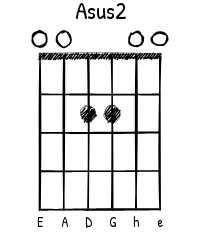
\includegraphics[height=3.5cm]{images/Asus2.png}
    \end{center}
    \vfill\null\columnbreak{}
    \begin{verse}
        Dzielny był przez tyle lat \\
        ``Czarnej Kuli'' nosił znak \\
        Imię jego wśród liniowców każdy znał \\
        Gdy na cumach w porcie stał \\
        Smukłe linie, piękny kształt \\
        Każdy morze razem z nim zdobywać chciał
    \end{verse}
    \begin{chorus*}
        Płynąć tam, gdzie czeka znów \\
        Żagli biel i silny wiatr \\
        Płynąć tam, gdzie żywioł, który wciąż nas gna \\
        Gdzieś do postrzępionych palm \\
        Do milczących, złotych plaż \\
        Dziś na pokład stary wrak nie weźmie nas
    \end{chorus*}
    \begin{verse}
        To wędrówki jego kres \\
        Skończył się już żagli wiek \\
        Nie powrócą pod błękitny nieba dach \\
        Tylko w sercach naszych trwa \\
        Do żaglowców z tamtych lat \\
        Wielka miłość, która w morze ciągnie nas
    \end{verse}
    \begin{chorus*}
        Chcemy płynąć tam, gdzie znów \\
        Żagli biel i silny wiatr \\
        Chcemy płynąć w żywioł, który wciąż nas gna \\
        Tam do postrzępionych palm \\
        Do milczących, złotych plaż \\
        Stary wrak wciąż pływać będzie w naszych snach
    \end{chorus*}
    \begin{interlude}
        Tam do postrzępionych palm \\
        Do milczących, złotych plaż \\
        Stary wrak wciąż pływać będzie w naszych snach
    \end{interlude}
    \end{multicols}
\end{song}


\newpage
\fancyfoot[LO,RE]{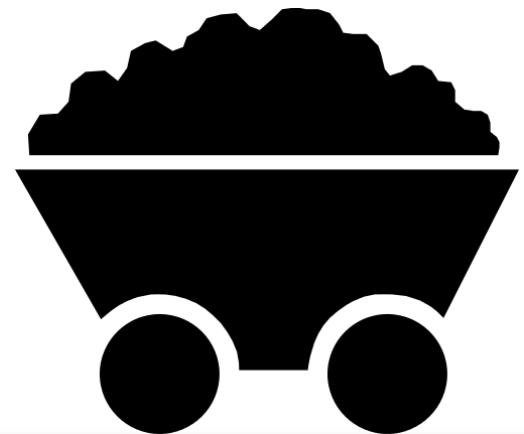
\includegraphics[height=45pt]{images/miner_cart.png}}
\begin{song}{title={Szesnaście ton}, music={Merle Travis}, lyrics={Marek Szurawski}}
    \begin{intro}
        \writechord{e}
    \end{intro}
    \begin{verse}
        Ktoś ^{e}mówił, że z gliny u^{e}lepił mnie Pan  \\
        A ^{e}przecież się składam z ^{e}kości i krwi  \\
        Z ^{e}kości i krwi, ^{a}jarzma na kark \\
        I ^{H7}pary rąk, pary ^{e}silnych rąk
    \end{verse}
    \begin{chorus}
        Co dzień szes^{e}naście ton, i ^{e}co z tego mam \\
        Tym ^{e}więcej mam długów, im ^{e}więcej mam lat \\
        Nie ^{e}wołaj Święty Piotrze, j^{a}a nie mogę przyjść \\
        Bo ^{H7}duszę swoją od^{C7}dałem za ^{e}dług\footnotemark{}
    \end{chorus}
    \begin{verse}
        Gdy matka mnie rodziła, pochmurny był dzień \\
        Więc wziąłem szuflę, poszedłem pod szyb \\
        Nadzorca mi rzekł: \say{Nie zbawi cię Pan  \\
        Załaduj co dzień szesnaście ton}
    \end{verse}
    \begin{chorus}
        Co dzień szesnaście ton\ldots
    \end{chorus}
    \begin{verse}
        Czort może dałby radę, a może i nie \\
        Szesnastu tonom podołać co dzień \\ 
        Szesnaście ton, szesnaście jak drut \\
        Codziennie nie da rady nawet dwóch
    \end{verse}
    \begin{chorus}
        Co dzień szesnaście ton\ldots
    \end{chorus}
    \begin{verse}
        Gdy kiedyś spotkasz mnie, lepiej z drogi mi zejdź \\
        Bo byli już tacy --- nie pytaj, gdzie są  \\
        Nie pytaj, gdzie są, bo zawsze jest ktoś \\
        Nie ten, to ów, co urządzi cię
    \end{verse}
    \begin{chorus}
        Co dzień szesnaście ton\ldots
    \end{chorus}
    \footnotetext{monopol w miasteczkach górniczych w USA powodował, że koszty życia przewyższały zarobki}
\end{song}

\newpage\pagestyle{szanty}
\newpage
\begin{song}{title={Szkuner „I'm Alone“}, music={Smugglers}}
    \small
    \begin{intro}
        \writechord{C} \writechord{a} \writechord{e}
    \end{intro}
    \begin{verse}
        Baksz^{e}tagiem pruł nasz \say{I'm Alone} hen, ^{G}od Meksyku b^{D}ram \\
        A ^{a}jankes, w dziób kopany, po ^{e}piętach deptał nam \\
        Ty^{e}siące beczek ^{G}rumu, od lo^{D}kerów aż po dno \\
        I ^{a}nawet kabla luzu, choćbyś r^{e}obił nie wiem co
    \end{verse}
    \begin{chorus}
        Sam ^{C}Neptun śpiewał szanty, po ^{G}cichu sprzyjał nam \\
        Więc ^{a}bił rekordy \say{I'm Alone}, choć g^{H7}roził wciąż Wuj Sam \\
        Na ^{C}jedną kartę wszystko, jak s^{G}truna k^{H}ażdy ^{e}bras \\
        \say{Niech di^{a}abli porwą Coast Guard} --- tak ^{e}mawiał każdy z nas
    \end{chorus}
    \begin{verse}
        A dawniej szkuner \say{I'm Alone} hen, po łowiskach gnał \\
        Lecz w końcu ryb zabrakło i głód w oczy zajrzał nam \\
        Za burty poszły sieci, bo tak krzyczał kobiet tłum \\
        Jankesi mają ginu dość, postawmy więc na rum
    \end{verse}
    \begin{chorus}
        Sam Neptun śpiewał szanty, po cichu sprzyjał nam\ldots
    \end{chorus}
    \begin{verse}
        Gdy stawialiśmy żagle, to Coast Guard wpadał w trans \\
        Ta banda bubków w baliach nie miała żadnych szans \\
        Pułapki zastawili, gnoje, choć tak dobrze szło \\
        Posłali dzielny \say{I'm Alone} z ładunkiem aż na dno
    \end{verse}
    \begin{verse*}
        Niejeden z Nowej Szkocji szkuner taki spotkał los \\
        A wszystko przez cholerny głód i wiecznie pusty trzos \\
        Lecz jeden z nich, nasz \say{I'm Alone} swe miejsce w pieśni ma \\
        I pewnie Neptun lubi go i w kości na nim gra
    \end{verse*}
    \begin{chorus}
        I nawet śpiewa szanty, po cichu sprzyja nam \\
        Choć leży na dnie \say{I'm Alone} i śmieje się Wuj Sam \\
        Na jedną kartę wszystko, jak struna każdy bras \\
        \say{Niech diabli porwą Coast Guard} --- tak mawiał każdy z nas
    \end{chorus}
    \begin{verse}
        A ci, co pokład \say{I'm Alone} kochali, jak swój dom \\
        Nie dla nich blaski sławy i nie dla nich w niebie tron \\
        Niech mają choć ten cichy klang, ten jeden marny dzwon \\
        I niech każdy do nich woła: \say{Hej, smuggler z \say{I'm Alone!}}
    \end{verse}
    \begin{chorus}
        Niech Neptun śpiewa szanty, po cichu sprzyja nam \\
        Rekordy bije \say{I'm Alone} i zamknie się Wuj Sam \\
        Na jedną kartę wszystko, jak struna każdy bras \\
        \say{Niech smuggler pije tylko rum!} --- tak mawia każdy znas $\times 2$
    \end{chorus}
    \begin{outro}
        \writechord{C} \writechord{a} \writechord{e}
    \end{outro}
\end{song}



\chapter{Poezja śpiewana}
\begin{center}
    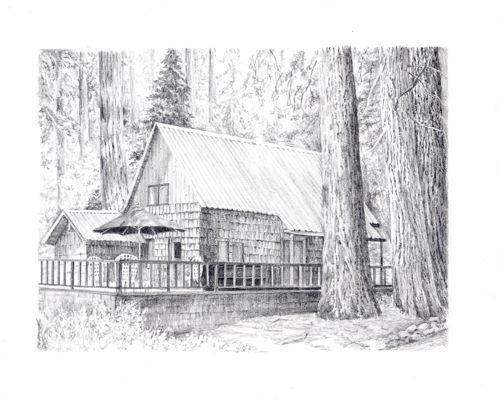
\includegraphics[width=0.5\textwidth]{images/chatka.jpg}
\end{center}
\pagestyle{poezja}
\newpage
\begin{song}{title={Ballada na złe drogi}, music={EKT Gdynia}}
\begin{multicols}{2}
    \begin{intro}
        \writechord{a} \writechord{F} \writechord{d} \writechord{E} $\times 2$
    \end{intro}
    \begin{verse}
        ^{d} Na drogi złe, ^{E}dni zwyczajne \\
        ^{a} I na najwyższe ^{F} z progów \\
        ^{d} Dostaliśmy w ^{E}dłonie balladę \\
        ^{a} I pachnie jak ^{A}owoc głogu
    \end{verse}
    \begin{chorus}
        ^{d} I będzie prze^{G}biegać muzyka \\
        Czy ty ^{C}wiesz, jak to dużo po dniu ^{F} \\
        ^{d} I w wierszu nam ^{E}będzie rozkwitać \\
        Bal^{a}lada --- posag m^{A}ój \\
        ^{d} I będzie prze^{G}biegać muzyka \\
        Czy ty ^{C}wiesz, jak to dużo po dniu ^{F} \\
        ^{d} I w wierszu nam ^{E}będzie rozkwitać ballada 
    \end{chorus}
    \begin{interlude}
        \writechord{a} \writechord{F} \writechord{d} \writechord{E} $\times 2$
    \end{interlude}
    \vfill\null{}
    \columnbreak{}
    \begin{verse}
        Na ludzi o szarych obliczach \\
        Na ścieżki i wilcze doły \\
        Gdy zechcę, na głos będzie krzyczeć \\
        I w miejscu nam nie ustoi
    \end{verse}
    \begin{chorus}
        I będzie przebiegać muzyka\ldots
    \end{chorus}
    \begin{interlude}
        \writechord{a} \writechord{F} \writechord{d} \writechord{E} $\times 2$
    \end{interlude}
    \begin{verse}
        A kiedy będziemy odchodzić \\
        Hen, do Krainy Łowów \\
        Błękitne się niebo otworzy \\
        I spadnie jak owoc głogu
    \end{verse}
    \begin{chorus}
        I będzie przebiegać muzyka\ldots
    \end{chorus}
    \begin{interlude}
        \writechord{a} \writechord{F} \writechord{d} \writechord{E} $\times 2$
    \end{interlude}
\end{multicols}
\end{song}


\newpage
\begin{song}{title={Dni, których nie znamy}, music={Jan Kanty Pawluśkiewicz}, lyrics={Marek Grechuta}, capo=3}
%\begin{multicols}{2}
    \begin{intro}
   		\textit{akordy jak w zwrotce}
   	\end{intro}
   	\begin{verse}
   		^{a}Tyle było ^{C}dni d^{G}o utraty s^{C}ił \\
		^{d}Do utraty t^{A}chu t^{C}yle było chw^{G}il \\
		^{a}Gdy żałujesz t^{C}ych z któ^{G}rych nie masz ^{C}nic \\
		^{d}Jedno warto zn^{A}ać je^{C}dno tylko wie^{G}dz
   	\end{verse}
   	\begin{chorus}
   		Że w^{F}ażne są tyl^{d}ko te dni^{E7}, których jes^{a}zcze nie zn^*{F}a m^{G}y ^{C} \\
		Ważnych jest kilka tych chwil, tych, na które czekamy \\
		Ważne są tylko te dni, których jeszcze nie znamy \\
		Ważnych jest kilka tych chwil, tych, na które czekamy
   	\end{chorus}
   	\begin{verse}
   		Pewien znany ktoś kto miał dom i sad \\
		Zgubił nagle sens i w złe kręgi wpadł \\
		Choć majątek prysł on nie stoczył się \\
		Wytłumaczyć umiał sobie wtedy właśnie, że 
   	\end{verse}
   	\begin{chorus}
   		Ważne są tylko te dni, których jeszcze nie znamy \ldots
   	\end{chorus}
   	\begin{interlude}
   		^{a}Jak rozpoznać lu^{G}dzi ^{C}których już nie zn^{G}amy \\
	   	^{a}Jak pozbierać my^{G}śli ^{C}z tych nieposkład^{G}anych \\
	   	^{d}Jak oddzielić na^{A}gle ^{F}serce od ro^{C}zumu \\
   		^{a}Jak usłyszeć si^{G}ebie ^{C}pośród śpiewu tł^{G}umu \\
		Jak rozpoznać ludzi których już nie znamy \\
		Jak pozbierać myśli z tych nieposkładanych \\
		Jak odnaleźć nagle radość i nadzieje \\ 
		Odpowiedzi szukaj czasu jest tak wiele
   	\end{interlude}
   	\begin{chorus}
   		Ważne są tylko te dni, których jeszcze nie znamy \ldots
   	\end{chorus}
%\end{multicols}
\end{song}
\fancyfoot[LO,RE]{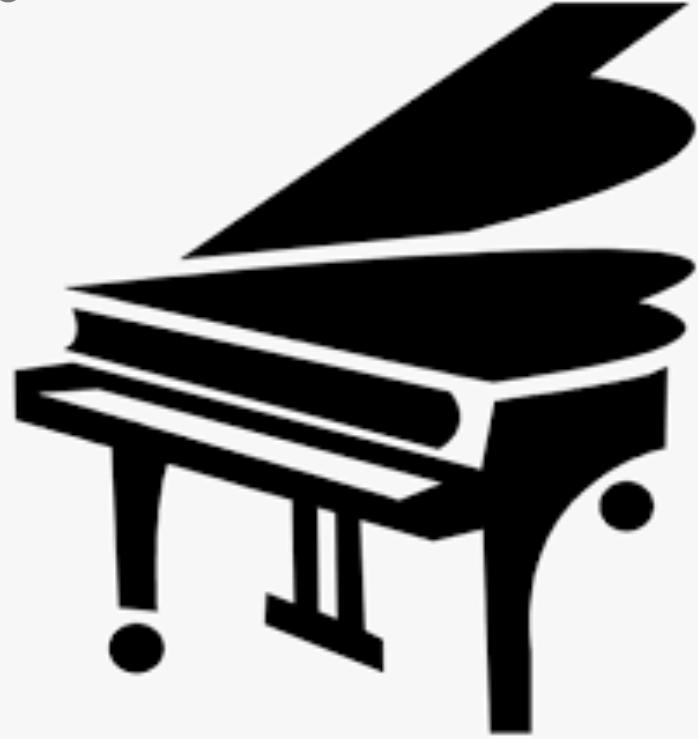
\includegraphics[width=2cm]{images/piano.png}}

\newpage\pagestyle{poezja}
\newpage
\begin{song}{title={Jak}, lyrics={Edward Stachura}, music={Stare Dobre Małżeństwo}}
    \begin{intro}
        \writechord{C}
    \end{intro}
    \begin{verse*}
        ^{C}Jak po nocnym niebie su^{G}nące białe ob^{F}łoki nad l^{C}asem \\
        Jak na ^{d}szyi wędrowca apa^{F}szka szamotana wi^{C}atrem 
    \end{verse*}
    \begin{verse*}
        Jak wyciągnięte tam powyżej gwiaździste ramiona wasze \\
        A tu są nasze, a tu są nasze
    \end{verse*}
    \begin{verse*}
        Jak suchy szloch w tę dżdżystą noc \\
        Jak winny-li-niewinny sumienia wyrzut \\
        Że się żyje, gdy umarło tylu, tylu, tylu 
    \end{verse*}
    \begin{verse*}
        Jak suchy szloch w tę dżdżystą noc \\
        Jak lizać rany celnie zadane \\
        Jak lepić serce w proch potrzaskane
    \end{verse*}
    \begin{verse*}     
        Jak suchy szloch w tę dżdżystą noc \\
        Pudowy kamień, pudowy kamień \\
        Ja na nim stanę, on na mnie stanie \\
        On na mnie stanie, spod niego wstanę 
    \end{verse*}
    \begin{verse*}
        Jak suchy szloch w tę dżdżystą noc \\
        Jak złota kula nad wodami \\
        Jak świt pod spuchniętymi powiekami
    \end{verse*}
    \begin{verse*}
        Jak zorze miłe, śliczne polany \\
        Jak słońca pierś, jak garb swój nieść \\
        Jak do was, siostry mgławicowe, ten zawodzący śpiew
    \end{verse*}
    \begin{verse*}
        Jak biec do końca, potem odpoczniesz, potem odpoczniesz \\
        Cudne manowce, cudne manowce, cudne, cudne manowce $\times 2$
    \end{verse*}
    \begin{verse*}
        Na na na na na, na na na \\
        Na na na, na na na na \\
        Na na, na na na na \\
        Na na na na
    \end{verse*}
    \begin{verse*}
        Jak biec do końca, potem odpoczniesz, potem odpoczniesz \\
        Cudne manowce, cudne manowce, cudne, cudne manowce $\times 2$
    \end{verse*}
    \begin{verse*}
        \textit{wolniej} \\
        Jak biec do końca, potem odpoczniesz, potem odpoczniesz \\
        Cudne manowce, cudne manowce, cudne, cudne manowce
    \end{verse*}
\end{song}


\newpage
\begin{song}{title={Jaka jesteś}, music={Tomasz Lewandowski}}
	\begin{intro}
	\writechord{G} \writechord{a} \writechord{C} \writechord{D} $\times 2$
	\end{intro}    
    \begin{verse}
        Jesteś ^{G}bitwą moją ni^{a}eskończoną \\
        ^{C} W której ciągle ^{D} o przyczułek wa^{G}lczę ^{a} ^{C} ^{D} \\
        Jesteś ^{G}drzwiami, które o^{a}tworzyłem \\
        ^{C} A potem ^{D} przycięły mi p^{G}alce ^{a} ^{C} ^{D}
    \end{verse}
  	\begin{chorus}
        Jesteś ^{G}kartką z kalendarza ^{a} \\
        Zagub^{C}ioną gdzieś pomię^{D}dzy szuflad^{G}ami ^{a} ^{C} ^{D} \\
        I u^{G}licą, na któ^{a}rej co dzień \\
        ^{C} Uciekałem mi^{D}ędzy latar^{G}niami ^{a} ^{C} ^{D}
    \end{chorus}
    \begin{verse}
        Jesteś mgłą ogromną niezmierzoną \\
        Ciszą w huku i łoskotem w ciszy \\
        Jesteś piórem i wyblakłą kartką \\
        Którym i na której dzisiaj piszę
    \end{verse}
    \begin{chorus}
        Jesteś kartką z kalendarza\ldots
    \end{chorus}
    \begin{interlude}
        \writechord{G} \writechord{F} \writechord{C} \writechord{D} $\times 2$
    \end{interlude}
    \begin{verse}
        Przyszłaś do mnie, a ja nie spostrzegłem \\
        Dzisiaj tylko mogę mówić: \say{Byłaś\ldots} \\
        Nie wiem czy na jawie wzięłaś mnie za rękę \\
        Czy jak wszystko ty się tylko sniłaś
    \end{verse}
    \begin{chorus}
        Że jesteś kartką z kalendarza\ldots $\times 2$
    \end{chorus}
\end{song}


\newpage
\begin{song}{title={Jest już za późno}, lyrics={Edward Stachura}, music={Stare Dobre Małżeństwo}}
    \begin{intro}
        \writechord{C} \writechord{F} \writechord{C} \writechord{F} 
    \end{intro}
    \begin{verse}
        ^{C}Jeszcze zdążymy w dżu^{d}ngli ludzkości ^{C}siebie odnaleźć ^{F} ^{C} \\
        ^{F} Tęskność zawr^{C}otna przybliża n^{d}as ^{G} \\
        ^{C}Zbiegną się wreszcie to^{d}ry sieroce n^{C}aszych dwóch planet ^{F} ^{C} \\
        ^{F} Cudnie spokr^{C}ewnią się ciała n^{d}am ^{G}
    \end{verse}    
    \begin{chorus}
        ^{e}Jest już za późno \\
        ^{F}Nie jest za późno \\
        ^{e}Jest już za późno \\
        ^{F}Nie jest za późno \\
        ^{e}Jest już za późno \\
        ^{F}Nie jest za ^{G}późno $\times 2$
    \end{chorus}
    \begin{verse}
        Jeszcze zdążymy tanio wynająć małą mansardę \\
        Z oknem na rzekę lub też na park \\
        Z łożem szerokim, piecem wysokim, ściennym zegarem \\
        Schodzić będziemy codziennie w świat 
    \end{verse}
    \begin{chorus}
        Jest już za późno\ldots $\times 2$
    \end{chorus}
    \begin{verse}
        Jeszcze zdążymy naszą miłością siebie zachwycić \\ 
        Siebie zachwycić i wszystko w krąg \\
        Wojna to będzie straszna, bo czas nas będzie chciał zniszczyć \\
        Lecz nam się uda zachwycić go
    \end{verse}
     \begin{chorus}
        Jest już za późno\ldots $\times 2$
    \end{chorus}
\end{song}


\newpage
\begin{song}{title={Majster Bieda}, lyrics={Wojciech Bellon}, music={Wolna Grupa Bukowina}, capo=2}
    \small
    \begin{intro}
        (\writechord{G}) \writechord{C} \writechord{F} \writechord{e} \writechord{d} $\times 2$ \\
        (\writechord{G}) \writechord{C}
    \end{intro}
    \begin{multicols}{2}
    \begin{verse}
        ^{C} Skąd przychodził, k^{d}to go znał \\
        K^{C}to mu ^{C7}rękę ^{F}podał ki^{G}edy \\
        Nad ^{C}rowem siadał, wyj^{G}mował chleb \\
        ^{e}Serem przekładał i ^{a}dzielił się z psem \\
        ^{G}Tyle wszystkiego, co z ^{F}sobą miał ^{e}--- ^{d} \\
        ^{G}Majster ^{C}Bieda ^{F} ^{e} ^{d}
    \end{verse}
    \begin{verse*}
        \writechord{G} \writechord{C}
    \end{verse*}
    \begin{verse}
        Czapkę z głowy ściągał, gdy \\
        Wiatr gałęzie chylił drzewom \\
        Śmiał się do słońca i śpiewał do gwiazd \\
        Drogę bez końca, co przed nim szła \\
        Znał jak pięć palców, jak szeląg zły --- \\
        Majster Bieda
    \end{verse}
    \begin{verse}
        Nikt nie pytał, skąd się wziął \\
        Gdy do ognia się przysiadał \\
        Wtulał się w krąg ciepła jak w kożuch \\
        Zmęczony drogą wędrowiec Boży \\
        Zasypiał długo, gapiąc się w noc --- \\
        Majster Bieda
    \end{verse}
    \vfill\null\columnbreak{}
    \begin{verse}
        Aż nastąpił taki rok \\
        Smutny rok, tak widać trzeba \\
        Nie przyszedł Bieda zieloną wiosną \\
        Miejsce, gdzie siadał, zielskiem zarosło \smallskip \\
        ^{G} I choć niejeden wy^{F}tężał wzrok \\
        Choć ^{G}lato pustym goś^{F}cińcem przeszło \\
        ^{G} Z rudymi liścmi, je^{F}sieni schedą \\
        ^{G}Wiatrem niesiony po^{F}płynął w przeszłość \\
        ^{G}Wiatrem niesiony po^{F}płynął w przeszłość \\
        ^{G}Wiatrem niesiony po^{F}płynął w ^{G}przeszłość --- \\
        ^{G}Majster ^{C}Bieda ^{F} ^{e} ^{d}
    \end{verse}
    \begin{verse*}
        \writechord{G} \writechord{C} \writechord{F} \writechord{e} \writechord{d} \\
        \writechord{G} \writechord{C}
    \end{verse*}
    \end{multicols}
\end{song}


\newpage
\normalsize
\begin{song}{title={Nim wstanie dzień}, music={Krzysztof Komeda}, lyrics={Agnieszka Osiecka}}
\begin{multicols}{2}
	\begin{intro}
		Ze ^{a}świata c^{e}zterech s^{a}tron \\
		Z ja^*{a}r zębi^{e}nowych dr^{a}óg \\
   		Gdzie l^{a}as spal^{e}ony, wi^{a}atr zmęczony, n^{D}oc i fr^{a}ont \\
   		Gdzie ni^{a}e zebr^{G}any pl^{a}on, gdzie ^{D}poczerniały gł^{a}óg \\
   		Wst^{e}aje dzi^{a}eń
	\end{intro}
	\begin{verse}
		Sł^{a}ońce przyt^{G}uli nas d^{a}o swych rąk i spójrz \\ 
		Ziemia ci^{D}ężka od kr^{a}wi \\
		Zno^{a}wu ur^{G}odzi nam zb^{a}oża ł^{G}an, złoty ku^{a}rz \\
		Przy^{a}jmą kobi^{G}ety nas p^{a}od swój dach i spójrz \\
		Będą śmi^{D}ać się przez ł^{a}zy \\
		Znowu do ta^{G}ńca ktoś za^{a}gra n^{G}am  \\
		Może j^{C}uż ^{E} 
	\end{verse}
	\begin{chorus}
		Za dzi^{a}eń, za d^{G}wa \\
		Za n^{G/H}oc, za t^{C}rzy \\
		Ch^{E}oć nie dz^{a}iś \\
		Za n^{a}oc, za dz^{G}ień \\
		Docz^{G/H}ekasz s^{C}ię \\
		Wst^{E}anie św^{a}it
	\end{chorus}
	\begin{verse}
		Chleby upieką się w piecach nam i spójrz  \\
		Tam, gdzie tylko był dym \\
		Kwiatem zabliźni się wojny ślad, barwą róż \\
		Dzieci urodzą się nowe nam i spójrz  \\
		Będą śmiać się, że my  \\
		Znów wspominamy ten podły czas, porę burz \\
	\end{verse}
	\begin{chorus}
		Za dzień, za dwa \ldots
	\end{chorus}
\end{multicols}
\end{song}


\newpage
\begin{song}{title={Pejzaże harasymowiczowskie}, lyrics={Wojciech Bellon}, music={Wolna Grupa Bukowina}}
    \begin{intro}
        \writechord{G} $\times 2$
    \end{intro}
    \begin{verse}
        ^{G} Kiedy wstałem w przed^{D}świcie, a Synaj \\
        ^{C} Prawdę głosił przez ^{e}trąby wiatru \\
        ^{G} Zasmreczyły się ^{D}chmury igliwiem \\
        ^{e} Bure świerki, o ^{C}góry wsp^{D}arte \medskip \\
        I na niebie byłem, ja jeden \\
        Plotąc pieśni w warkocze bukowe \\
        I schodziłem na ziemię za kwestą \\
        Przez skrzydlącą się bramę Lackowej
    \end{verse}
    \begin{chorus}
        ^{G} I był Beskid, i ^{C}były ^{G}słowa \\
        ^{G} Zanurzone po ^{C}pępki w cerkwi \\
        b^{D}aniach, rozło^{D}żyście złotych \\
        ^{C} Smagających się ^{D}wiatrem ^{G}do krwi \medskip \\
        \writechord{G}
    \end{chorus}
    \begin{verse}
        Moje myśli biegały końmi \\
        Po niebieskich, mokrych połoninach --- \\
        I modliłem się, złożywszy dłonie \\
        Do gór, do Madonny Brunatnolicej \smallskip \\
        A gdy serce kroplami tęsknoty \\
        Jęło spadać na góry sine  \\
        Czarodziejskim kwiatem paproci \\
        Rozgwieździła się bukowina
    \end{verse}
    \begin{chorus}
        I był Beskid, i były słowa\ldots
    \end{chorus}
\end{song}


\newpage
\begin{song}{title={Pójdę w połoniny (A ja wolę…)}, music={Dom o Zielonych Progach}}
    \begin{verse}
        ^{E} A ja ^{a}wolę \\
        ^{E} Na zielonej ^{a}łące ^*{G}sie ^{F}dzieć \\
        Niźli w ^{C}szarym mieście, które ^{E} głuche jest \\
        ^{F} Na moje wo^{C}łanie \\
        ^{F} Na mój niemy ^{C}krzyk \\
        ^{F} Na moją sa^{C}motność obo^{E}jętne ^{a}jest ^{G} ^{F} ^{C}
    \end{verse}
    \begin{verse}
        Pójdę w połoniny \\
        W roztańczone bujne trawy \\
        Pod rękę razem z polnym wiatrem \\
        Między szumem liści \\
        Ukryte słowa dla mnie \\
        Zanucę je głośniej, niech popłyną dalej gdzieś
    \end{verse}
    \begin{verse}
        Niech na moim niebie \\
        Rozniebieszczą się gwiazdy \\
        Niczym Mały Książę będę sobie szedł \\
        Może spotkam różę \\
        Której kolców brak \\
        Która zdradzi mi swe imię i swój uśmiech da
    \end{verse}
    \begin{interlude}
        Na na na na na\ldots
    \end{interlude}
    \begin{verse}
        Pójdę w połoniny\ldots
    \end{verse}
\end{song}


\newpage
\begin{song}{title={Sielanka o domu}, music={Wolna Grupa Bukowina}}
\begin{multicols}{2}
	\begin{intro}
		\writechord{G}
	\end{intro}
    \begin{verse}
        ^{G} A jeśli d^{a7}om będę m^{h7}iał ^{G7} \\
		To bę^{C}dzie buk^{D7}owy koni^{G}ecznie ^{Gmaj7} \\
		Pac^{a7   D7}hnący i sło^{h7    G}neczny \\
		Wiecz^{C}orem usi^{D}ądę wiatr gra \\
		A z^{G}egar na śc^{G7}ianie gwa^{C}rzy  ^{D} \\ 
		D^{G}obrze się ^{a7}idzie p^{h7}anie zeg^{G7}arze \\
		Tik t^{a7}ak, tik ta^{D7}k, tik t^{G   G7}ak \\
		Świeca skwi^{C}erczy i mruga przewr^{D}otnie \\
		Więc pu^{G}szczam ^{a7}oko d^{h7}o niej^{G7} \\
		Dobry h^{a7}umor dz^{D7}iś pani m^{G}a ^{G7} \\
		Dobry h^{a7}umor dz^{D7}iś pani ma ^{G}
    \end{verse}
    \begin{chorus}
    	^{G}Szukam szuk^{D}ania mi trzeba \\
		^{F}Domu git^{C}arą i pi^{G}órem \\ 
		^{G}A góry nade^{D} mną jak niebo  \\
		A ^{F}niebo nad^{C}e mn^{c}ą jak gó^{G}ry $\times 2$
    \end{chorus}
    \begin{verse}
        Gdy głosy usłyszę u drzwi \\
		Czyjekolwiek wejdźcie poproszę \\
		Jestem zbieraczem głosów \\
		A dom mój bardzo lubi gdy \\
		Śmiech ściany mu rozjaśnia \\
		I gędźby lubi pieśni \\
		Wpadnijcie na parę chwil \\
		Kiedy los was zawiedzie w te strony \\
		Bo dom mój otworem stoi \\
		Dla takich jak wy \\
		Dla takich jak wy
    \end{verse}
    \begin{chorus}
    	Szukam szukania mi trzeba \ldots $\times 2$
    \end{chorus}
    \begin{verse}
        Zaproszę dzień i noc \\
		Zaproszę cztery wiatry \\
		Dla wszystkich drzwi otwarte \\
		Ktoś poda pierwszy ton \\
		Zagramy na góry koncert \\ 
		Buków porą pachnącą \\
		Nasiąkną ściany grą \\
		A zmęczonym wędrownikom \\
		Odpocząć pozwolą muzyką \\
		Bo taki będzie mój dom \\ 
		Bo taki będzie mój dom \\
		Bo taki będzie mój dom
    \end{verse}
    \begin{chorus}
    	Szukam szukania mi trzeba \ldots $\times 2$
    \end{chorus}
\end{multicols}
\end{song}


\newpage
\fancyfoot[LO,RE]{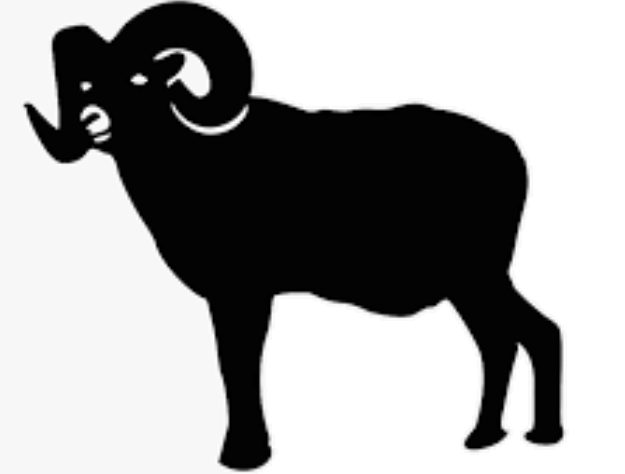
\includegraphics[width=2cm]{images/baran.png}}
\begin{song}{title={Świecie nasz}, music={Jan Kanty Pawluśkiewicz}, lyrics={Marek Grechuta}, annex}
\begin{multicols}{2}
    \begin{intro}
        \writechord{g} \writechord{F} \writechord{Eb} \writechord{d}
    \end{intro}
    \begin{verse}
        ^{g} Pytać zawsze --- ^{F}dokąd, dokąd \\
        ^{Eb} Gdzie jest prawda, ^{d}ziemi sól \\
        ^{g} Pytać zawsze --- ^{F}jak zagubić \\
        ^{Eb} Smutek wszelki, ^{d}płacz i ból
    \end{verse}
    \begin{verse}
        ^{g} Chwytać myśli n^{F}agłe, jasne \\
        ^{B} Szukać tam, gdzie świ^{F/A}atła biel \\
        |: ^{g} W Twoich oczach d^{F}wa ogniki | \\
        | ^{Eb} Już zwiastują, z^{d}naczą cel :|
    \end{verse}
    \begin{verse*}
        \writechord{g} \writechord{F} \writechord{Eb} \writechord{d} \\
        \writechord{g} \writechord{F} \writechord{Eb} \writechord{d} \\
        \writechord{g}
    \end{verse*}
    \begin{interlude}
        ^{a} Świecie nasz, ^{g}świecie nasz \\
        Chcę być z Tobą w ^{d}zmowie \\
        ^{F} Z blaskiem Twym, ^{d6}siłą twą \\
        Co mi dasz? Odp^{asus2}owiedz ^{A}
    \end{interlude}
    \begin{info}
        Świecie nasz --- daj nam \\
        Daj nam wreszcie zgodę \\
        Spokój daj --- zgubę weź \\
        Zabierz ją, odprowadź
    \end{info}
    \begin{info}
        Szukaj dróg gdzie jasny dźwięk \\
        Wśród ogni złych co budzą lęk \\
        Nie prowadź nas, powstrzymaj nas \\
        Powstrzymaj nas w pogoni\ldots
    \end{info}
    \begin{chorus}
        ^{F}Świecie ^{C}nasz \\
        Daj nam wi^{d}ele jasnych dni \\
        ^{a}Świecie n^{F}asz \\
        Daj nam w j^{G}asnym dniu oczekiwanie \medskip \\
        Świecie nasz \\
        Daj ugasić ogień zły \\
        Świecie nasz \\
        Daj nam radość, której tak szukamy \\
        Świecie nasz \\
        Daj nam płomień, stal i dźwięk \\
        Świecie nasz \\
        Daj otworzyć wszystkie ciężkie bramy \\
        Świecie nasz \\
        Daj pokonać każdy lęk \\
        Świecie nasz \\
        Daj nam radość blasku i odmiany! \\
        Świecie nasz \\
        Daj nam cień wysokich traw \\
        Świecie nasz \\
        Daj zagubić się wśród drzew poszumu \\
        Świecie nasz \\
        Daj nam ciszy czarny staw \\
        Świecie nasz \\
        Daj nam siłę krzyku, śpiewu tłumu \\
        Świecie nasz \\
        Daj nam wiele jasnych dni \\
        Świecie nasz \\
        Daj nam w jasnym dniu oczekiwanie \\
        Świecie nasz \\
        Daj ugasić ogień zły \\
        Świecie nasz
    \end{chorus}
    \begin{outro}
        Świecie nasz, świecie nasz \\
        Chcę być z tobą w zmowie \\
        Z blaskiem twym, z siłą twą \\
        Co mi dasz? Odpowiedz
    \end{outro}
\end{multicols}
\end{song}
\newpage\pagestyle{poezja}
\newpage
\begin{song}{title={Wilcza zamieć}, music={Marcin Przybyłowicz (z gry Wiedźmin: Dziki Gon)}, interpret={Studio Accantus}}
    \begin{intro}
        \writechord{d} \writechord{d} \writechord{B} \writechord{C} $\times 2$
    \end{intro}
    \begin{verse}
        Na ^{d}szlak moich blizn po^{B}prowadź ^{C}palec \\
        By ^{d}nasze drogi spleść ^{g}gwiazdom na ^{A}przekór \\
        ^{B} Otwórz te rany, ^{g} a potem ^{A}zalecz \\
        ^{d}Aż w zawiły losu ułożą się wzór
    \end{verse}
    \begin{chorus}
        Z moich ^{d}snów uciekasz nad ranem \\
        Cierpka ^{B}jak agrest, słodka jak bez ^{C} \\
        Chcę ^{d}śnić czarne loki splątane \\
        ^{B}Fiołkowe oczy ^{g}mokre od ^{A}łez
        \\
    \end{chorus}
    \begin{verse}
        Za wilczym śladem podążę w zamieć \\
        I twoje serce wytropię uparte \\
        Przez gniew i smutek stwardniałe w kamień \\
        Rozpalę usta smagane wiatrem
    \end{verse}
    \begin{chorus}
        Z moich snów uciekasz nad ranem\ldots
    \end{chorus}
    \begin{verse}
        Nie wiem czy jesteś moim przeznaczeniem \\
        Czy przez ślepy traf miłość nas związała \\
        Kiedy wyrzekłem moje życzenie \\
        Czyś mnie wbrew sobie wtedy pokochała?
    \end{verse}
    \begin{chorus}
        Z moich snów uciekasz nad ranem\ldots
    \end{chorus}
    \begin{interlude}
        \writechord{d} \writechord{d} \writechord{B} \writechord{C} $\times 2$
    \end{interlude}
\end{song}


\newpage
\begin{song}{title={1788}, music={Jacek Kaczmarski}}
    \small
    \begin{intro}
        \writechord{F} \writechord{B} \writechord{F} \writechord{C} \\ 
        \writechord{F} \writechord{B} \writechord{F} \writechord{C} \writechord{F}
    \end{intro}
    \begin{multicols}{2}
\begin{verse}
^{F}Ta pierwsza morska ^{B}podróż do Australii! \\
^{F}Łotry przy burtach, prosty^{C}tutki w kojach \\
^{F}Wszyscy się bali, łk^{B}ali i rzygali \\
^{F}W drodze do raju. Przewrot^{C}ności Twoja \\
^{d}Panie, coś w jeszcze nam niezn^{g}anych planach \\
^{d} Miał czarne diabły strzeg^{a}ące wybrzeży \\
^{B}Edenu, który prz^{C}eznaczyłeś ^{F}dla nas \\
A w kt^{B}óry nikt, prawdę ^{C}mówiąc, nie ^{d}wierzył! \\
\\
^{d} ^{B} ^{F} ^{C}
\end{verse}
\begin{verse}
Czym żeśmy, marni, zasłużyli na to? \\
Ten, co zawisnąć miał za kradzież płaszcza \\
Płakał nad swoją niechybną zatratą \\
Nie widział Ciebie w robaczywych masztach \\
Statku, co tylko był więzieniem nowym \\
Tej co kupczyła ciałami swych dziatek \\ 
Ani przez mgnienie nie przyszło do głowy \\
Że to nadziei - nie rozpaczy statek \\
\end{verse}
\begin{verse}
Niejeden żołnierz z ponurej eskorty \\
Bo czym się ich los od naszego różnił? \\ 
Wiedział, że nigdy już nie ujrzy portu \\
Gdzie go podejmą karczmarze usłużni \\ 
I płatne dziewki; że zabraknie rumu \\
Zanim do celu przygnasz okręt szparki \\
Z marynarzami pili więc na umór \\
I - wbrew zakazom - grali o więźniarki \\
\end{verse}
\begin{verse}
Prawda, nie wszyscy próby Twe przetrwali \\
Ale też ciężkoś nas doświadczał, Panie \\
Nie oszczędzałeś nam wysokiej fali \\ 
Za którą mnogim przyszło w oceanie \\
Zakończyć żywot; innym dziąsła zgniły \\
Wypadły zęby, rozgorzały wrzody \\ 
Więc znaczą nasz zielony szlak mogiły \\
Szkorbutu, szału, francuskiej choroby \\
\end{verse}
\begin{verse}
Nikt nie odnajdzie w ruchomych otchłaniach \\
Ciał nieszczęśników - oprócz Ciebie, Boże \\
Ich żywot grzeszny epitafiów wzbrania \\
Lecz - ukarani. Więc wystarczy może \\ 
Żeś się posłużył straszliwym przykładem \\
Oni naprawdę dotarli do piekieł \\
A umierając nie wierzył z nich żaden \\
Że w swym cierpieniu umiera - człowiekiem \\
\end{verse}
\begin{verse}
Ląd nam się wydał niegościnny, dziki \\
Łotr bez honoru, kobieta sprzedajna \\
Z dnia na dzień - jak się stać ma osadnikiem \\
Nieznanych światów? Bo rozpoznać Raj nam \\
Nie było łatwo; znaleźć w sobie siłę \\
Wbrew przeciwnościom, bez słowa zachęty \\
By mimo wszystko żyć - nim nam odkryłeś \\ 
Kraj szczodry w zboże, złoto i diamenty \\
\end{verse}
\begin{verse}
^{d}Łajdacki pomiot, łot^{g}rowskie nasienie \\
^{d}Czerpiąc ze spichrza Twoich d^{a}óbr wszelakich \\
^{B}Choć tyle wiemy w^{C}łasnym doświadcz^{F}eniem \\
^{d}W nas jest Raj, Pi^{B}ekło - ^{F}I do obu-szl^{C}aki \\
^{d}W nas jest Raj, Pi^{B}ekło - ^{F}I do obu-szl^{C}aki \\
^{d}W nas jest Raj, Pi^{B}ekło - ^{F}I do obu-szl^{C}aki \\
\\
\writechord{d} \writechord{B} \writechord{F} \writechord{C}
\end{verse}
\end{multicols}
\begin{center}
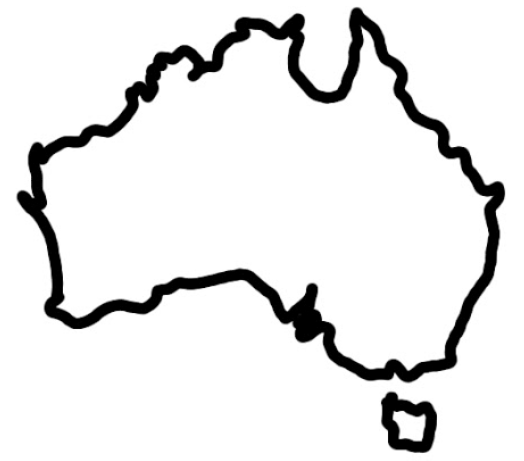
\includegraphics[width=0.15\textwidth]{images/1788.png}  
\end{center}
\end{song}
\newpage
\newpage\pagestyle{poezja}

\chapter{Pop}
\begin{center}
    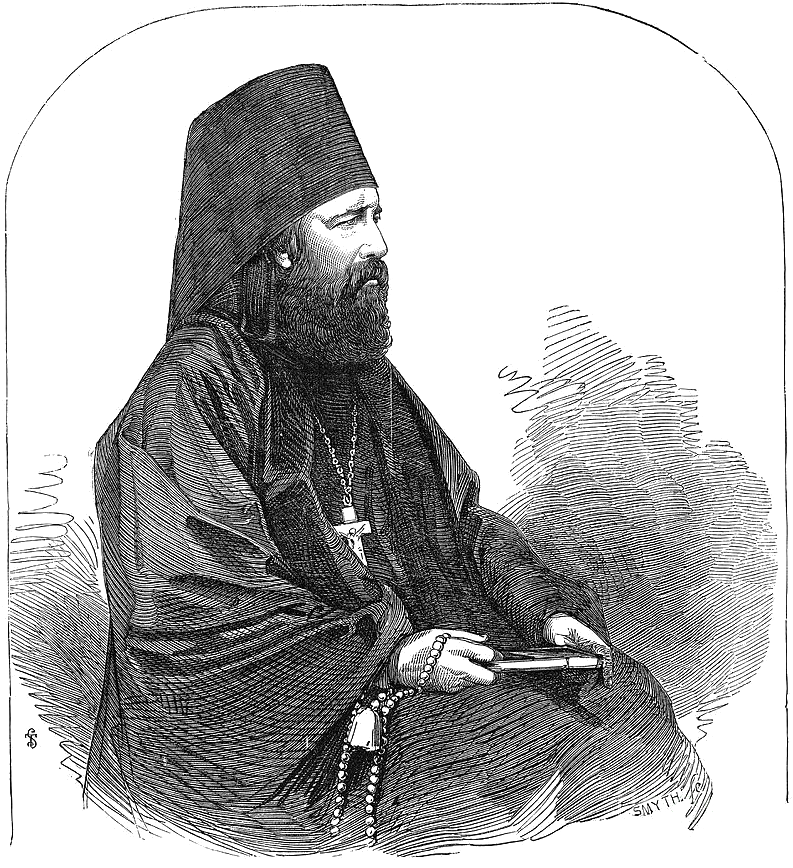
\includegraphics[width=0.4\textwidth]{images/pop.png}
\end{center}
\pagestyle{pop}
\newpage
\begin{song}{title={Byłaś serca biciem}, music={Jerzy Dobrzyński}, interpret={Andrzej Zaucha}, capo=3}
    \begin{intro}
    \writechord{a} \writechord{G} \writechord{d7} \writechord{d7}
    \end{intro}
    \begin{chorus}
        ^{a}Byłaś serca b^{G}iciem ^{d7} \\
        ^{a}Wiosną, zimą, ż^{G}yciem ^{d7} \\
        ^{a}Marzeń moich e^{G}chem ^{d7} \\
        ^{a}Winem, wiatrem, śmi^{G}echem ^{d7}
    \end{chorus}
    \begin{verse}
        Ostatnio w ^{a}mieście mym tramwaje ^{G}po północy b^{d7}łądzą \\
        Rozkładem n^{a}ocnych tras piekielne ^{G}jakieś moce rz^{d7}ądzą \\
        Nie wiedzieć ^{a}czemu wciąż rozkł^{G}ady jazdy ta^{d7}k zmieniają \\
        Że prawie k^{a}ażdy tramwaj ^{G}pod twym oknem ^{d7}nocą staje
    \end{verse}
      \begin{chorus}
        Byłaś serca biciem\ldots
    \end{chorus}
    \begin{verse}
        Ostatnio słońca mniej, ostatnio noce bardziej ciemne \\
        Już nawet księżyc drań o tobie nie chce gadać ze mną \\
        W kieszeni grosze dwa, w kieszeni na dwa szczęścia grosze \\
        W tym jednak losu żart, że ja obydwa grosze noszę
    \end{verse}
    \begin{chorus}
        Byłaś serca biciem\ldots
    \end{chorus}
    \begin{interlude}
        ^{F}Ktoś p^{d7}ytał jak się m^{C}asz, j^{a}ak się czujesz \\
        ^{F}Ktoś, z k^{d7}im rok w wojnę g^{C}rasz wycze^*{e}ku ^{A}je \\
        ^{F}Ktoś, k^{d7}to nocami, u^{C}licami, t^{a}ramwajami \\
        ^{F}Pod twe okno ^{d7}mknie, gdzie spo^*{D}ty ^{Eb}ka ^{E}mnie
    \end{interlude}
    \begin{chorus}
        Byłaś serca biciem\ldots
    \end{chorus}
    \begin{interlude}
        Ktoś pytał jak się masz\ldots
    \end{interlude}
\end{song}


\newpage
\begin{song}{title={Granda}, music={Monika Brodka}}
	\begin{intro}
	\writechord{e} \writechord{e} \writechord{H} \writechord{A} $\times 2$ \\
		Ni^{e}e polubię cię \\
		Jak powiedzieć prościej \\
		Zbl^{H}iżysz się o krok, porach^{A}uję kości \\
		Ni^{e}e polubię cię \\
		Twej koszuli pstrości \\
		Zbl^{H}iżysz się o krok, porach^{A}uję kości
	\end{intro}
	\begin{verse}
		\textit{riff:} \writechord {e5} \writechord{h5} \writechord{d5} \writechord{a5} \\	\\
		Kusisz zapachami \\
		Prowokujesz gestem \\
		Wodzisz za mną wzrokiem \\
		Czterogłowym smokiem \\
		Namierzasz radarami \\
		Jestem jak ruchomy cel \\
		Naostrzone zęby \\ 
		Nie polubię cię 
	\end{verse}
	\begin{chorus}
		Ni^{e}e polubię cię \\
		Jak powiedzieć prościej \\
		Zbl^{H}iżysz się o krok, porach^{A}uję kości \\
		Ni^{e}e polubię cię \\
		Twej koszuli pstrości \\
		Zbl^{H}iżysz się o krok, porach^{A}uję kości \\
		Do pięciu liczę, znikaj \\
		Dwa, trzy, cztery, pięć \\ 
		Raz, dwa, trzy, cztery, pięć \\
		Nie będzie dziś walczyka \\ 
		Dwa, trzy, cztery, pięć \\
		Raz, dwa, trzy, cztery, pięć \\
	\end{chorus}
	\begin{verse}
		Tropią mnie zwiadowcy \\
		Węszą myśliwskie psy \\
		Jak dziką zwierzynę \\
		Co kruszeje żywcem \\
		Zastawiłeś sidła \\
		Zmieniłeś zasady gry \\ 
		Zablokowałeś drogi \\
		Zaryglowałeś drzwi
	\end{verse}
	\begin{chorus}
		Nie polubię cię \ldots $\times 2$
	\end{chorus}
\end{song}


\newpage
\small
\begin{song}{title={In the End}, music={Linkin Park}, capo={1}}
    \begin{intro}
        \writechord{d} \writechord{C} \writechord{B} \writechord{C} $\times 2$
    \end{intro}
    \begin{multicols}{2}
    \begin{verse}
        \textit{(It starts with\ldots)} \\
        ^{d}One thing, I don't know why \\
        It ^{C}doesn't even matter how hard you try \\
        Ke^{B}ep that in mind, I designed this rhyme \\
        To expla^{C}in in due time \textit{(all I know)} \\
        Time is a valuable thing \\
        Watch it fly by as the pendulum swings \\
        Watch it count down to the end of the day \\
        The clock ticks life away \textit{(it's so unreal)} \\
        Didn't look out below \\
        Watch the time go right out the window \\
        Tryin' to hold on, I didn't even know \\
        I wasted it all, just to\ldots \textit{(watch you go)} \\
        I kept everything inside \\
        And even though I tried, it all fell apart \\
        What it meant to me will eventually be \\
        A memory of a time, when\ldots
    \end{verse}
    \begin{chorus}
        I tried so ^{d}hard and got so f^{F}ar \\
        But in the e^{C}nd, it doesn't even ma^{B}tter \\
        I had to ^{d}fall to lose it a^{F}ll \\
        But in the e^{C}nd, it doesn't even ma^{B}tter
    \end{chorus}
    \vfill\null\columnbreak{}
    \begin{verse}
        One thing, I don't know why \\
        It doesn't even matter how hard you try \\
        Keep that in mind, I designed this rhyme \\
        To remind myself how\ldots \textit{(I tried so hard)} \\
        In spite of the way you were mockin' me \\
        Actin' like I was part of your property \\
        Rememberin' all the times you fought with me \\
        I'm surprised it\ldots \textit{(got so far)} \\
        Things aren't the way they were before \\
        You wouldn't even recognize me anymore \\
        Not that you knew me back then \\
        But it all comes back to me \textit{(in the end)} \\
        You kept everything inside \\
        And even though I tried, it all fell apart \\
        What it meant to me will eventually be \\
        A memory of a time when\ldots
    \end{verse}
    \begin{chorus}
        I tried so hard and got so far\ldots
    \end{chorus}
    \begin{interlude}
        I've put my tr^{d}ust in yo^{C}u \\
        Pushed as f^{B}ar as I can g^{C}o \\
        For all th^{d}is, there's only o^{C}ne thing you should ^*{B}kn ^{C}ow
    \end{interlude}
    \begin{info}
        \textit{(mocniej, głośniej, \textbf{drzeć ryja})} \\
        I've put my tr^{d}ust in yo^{F}u \\
        Pushed as f^{C}ar as I can g^{B}o \\
        For all th^{d}is, there's only o^{F}ne thing you should ^*{C}kn ^{B}ow
    \end{info}
    \begin{chorus}
        I tried so hard and got so far\ldots
    \end{chorus}
    \begin{interlude}
        \writechord{d} \writechord{C} \writechord{B} \writechord{C} $\times 2$
    \end{interlude}
    \end{multicols}
\end{song}


\newpage
\begin{song}{title={Kolorowy wiatr}, music={Alan Menken}, lyrics={Antoni Marianowicz}}
\small
    \begin{info}
        \writechord{N.C.} --- \say{No Chord}, pauza
    \end{info}
    \begin{multicols}{2}
    \begin{intro}
        \writechord{c} \\
        Ty m^{c}asz mnie za głupią dzi^{c/B}kuskę \\
        Lecz choć c^{c}ały świat zwiedziłeś \\
        Zj^{B}eździłeś wzdłuż i wszerz \\
        I m^{G#}ądry jesteś ^{N.C.}tak \\
        Że aż sł^{G#}ów podziwu br^{N.C.}ak \\
        Dla^{f}czego powiedz mi tak mało wi^{G}esz \\
        Mało wi^{C}esz ^{a} ^{C} ^{a}
    \end{intro}
    \begin{verse}
        Na l^{C}ądzie gdy rozglądasz się lą^{a}dując \\
        Chcesz wsz^{C}ystko mieć na własność, nawet gł^{e}az \\
        A ^{F}ja wiem, że ten głaz ma także d^{a}uszę \\
        Imię m^{d}a i zakl^{G}ęty w sobie cz^{a}as \smallskip \\
        Ty m^{C}yślisz, że są ludźmi tylko l^{a}udzie \\
        Których l^{C}udźmi nazywać chce twój świ^{e}at \\
        Lecz j^{F}eśli pójdziesz tropem moich br^{a}aci \\
        Dowiesz ^{d}się największych pr^{G}awd \\
        Najświętszych pr^{C}awd
    \end{verse}
    \vfill\null\columnbreak{}
    \begin{chorus}
        Czy wiesz, cz^{a}emu wilk tak wyje w księżyc^{e}ową n^{F}oc \\
        I cze^{a}mu ryś tak zęby szczerzy ra^{e}d?  \\
        Czy powt^{F}órzysz te mel^{G}odie, co z gór pł^{C}yną ^{a} \\
        Barwy, kt^{d7}óre kolorowy niesie wi^{G}atr \\
        Barwy, kt^{F}óre kolor^{G}owy niesie wi^{C}atr ^{a} ^{C} ^{a}
    \end{chorus}
    \begin{verse}
        \textit{(szybciej)} \\
        Pobiegnij za mną leśnych duktów szlakiem \\
        Spróbujmy jagód w pełne słońca dni \\
        Zanurzmy się w tych skarbach niezmierzonych \\
        I choć raz o ich cenach nie mów mi \smallskip \\
        Ulewa jest mą siostrą, strumień bratem \\
        A każde z żywych stworzeń to mój druh \\
        Jesteśmy połączonym z sobą światem \\
        A natura ten krąg życia wprawia w ruch
    \end{verse}
    \begin{interlude}
        Do ch^{F}mur każde dr^{e}zewo się pn^{a}ie \\
        Skąd to wi^{d}edzieć masz, skoro ści^{G}nasz je
    \end{interlude}
    \begin{chorus}
        To nie to^{a}bie ptak się zwierza w księży^{e}cową n^{F}oc  \\
        Lecz lu^{a}dziom wszelkich ras i wszelkich wi^{e}ar \\
        Chło^{F}nącym te mel^{G}odie, co z gór pł^{C}yną ^{a} \\
        Barwy, kt^{d7}óre kolorowy niesie wi^{G}atr \\
        Możesz zd^{d}obyć św^{e}iat, lecz to bę^{d}dzie ty^{e}lko świ^{F}at \\
        Tylko św^{a}iat --- nie barwy, które ^*{d7}nie ^{Gadd2}sie wi^{C}atr
    \end{chorus}
    \end{multicols}
\end{song}


\newpage
\small
\begin{song}{title={Małociasteczkowy}, music={Dawid Podsiadło}, interpret={808 Squad}}
\begin{multicols}{2}
    \begin{intro}
        (\textit{jęcząc}) \\
        H^{h}u hu hu hu hu hu h^{A}u hu h^{D}uuu, hu \\
        H^{E}u hu h^{f#}uuu, hu \\
        Hu hu h^{E}uuu, hu
    \end{intro}
    \begin{verse}
        Małociasteczk^{A}owa twarz \\
        ^*{E}Małoci astecz^{D}kowa głowa \\
        ^*{E}Małoci asteczk^{A}owy styl \\
        ^*{E}Małoci astecz^{D}kowo kocham \\
        Z ma^{h}łego ciasta wielkie sny  ^{A/C#} \\
        Atak^{D}ują twoje ulice ^{E}  \\
        Wyś^{f#}niłem sobie ciebie, gdy \\
        Śpiew^{E}ałem głośno pod prysznicem
    \end{verse}
    \begin{verse}
        Ten mój małociasteczkowy hit \\
        I małociasteczkowe słowa \\
        Ten małociasteczkowy rytm \\
        Melodia małociasteczkowa \\
        Z małego ciasta wielkie sny \\
        Gromadzą się na twoich ulicach \\
        Pamiętam, bardzo chciałem tu być \\
        Na pewno dużo bardziej niż dzisiaj
    \end{verse}
    \begin{chorus}
        Zn^{f#}owu jadę d^{E}o ciebie s^{A}am ^{h} \\
        Zn^{D}owu jadę do ciebi^{c#}e ^{E} $\times 4$
    \end{chorus}
    \begin{verse}
        Przez chwilę czułem się jak Bóg \\
        Przez chwilę byłem królem w cieście \\
        Wybrałem na siłownię strój \\
        I wtedy zrozumiałem wreszcie \\
        Że z mojego ciasta moje sny \\
        Budują twoje ulice \\
        Że ciebie nie zachwyca tu nic \\
        Ale smuci mnie, że nadal nie krzyczę
    \end{verse}
    \begin{verse}
        Gdy wielkomiejski piękny świat \\
        Na każdym kroku sypie kreski \\
        Uściski i klepnięcia w bark \\
        Płynące ze wzruszenia łezki \\
        Dlaczego wszystko sztuczne aż tak \\
        Że napromieniowane mi świeci \\
        Trzeba stąd wyjechać, bo strach \\
        Że wszystko przejdzie na moje dzieci
    \end{verse}
    \begin{interlude}
        Hu hu hu hu\ldots $\times 2$
    \end{interlude}
    \begin{chorus}
        Znowu jadę do ciebie sam \\
        Znowu jadę do ciebie $\times 3$
    \end{chorus}
    \begin{outro}
        H^{f#}u hu hu hu h^{E}u hu h^{A}uuu, hu \\
        H^{h}u hu hu^{D}uu, hu \\
        Hu hu h^{c#}uu hu ^{E} $\times 2$
    \end{outro}
\end{multicols}
\end{song}


\newpage
\small
\begin{song}{title={Miał być ślub}, music={Bartłomiej Kapłoński}, lyrics={Anna Dąbrowska}, interpret={Monika Brodka}} 
    \begin{intro}
        \writechord{D}
    \end{intro}
    \begin{verse}
        ^{D}Żoną miałam b^{D7}yć, miał być ś^{G}lub i we^{g}sele też \\
        Już ^*{D}zapro ^{f#/C#}siłam g^{H7}ości, kap^{e}ela z r^{e7/D}odzinnych st^{A/C#}ron \\
        ^{h}Miała tam gr^{A}ać ^{G}polkę na d^{F#}wa \\
        Matki ^*{h}pobłogosław ^{E/G#}iły dawno ^{A} nam ^{A7/G} ^{f#} ^{A/E}
    \end{verse}
    \begin{verse}
        Był umówiony ksiądz, bukiet mi przywieźli z białych róż \\
        Welon już na głowie, kościół pęka w szwach \\
        Babcia we łzach cichutko łka \\
        Organista daje znak, a jego brak
    \end{verse}
    \begin{chorus}
        Su^{D}kienka sa^{F#}motnie w szafie lś^{h}ni, nie zał^{E}oży jej już ni^{A}kt \\
        ^{E/G#} Nie dowie s^{f#}ię \\
        ^{h}Czemu ^{A}tak stało s^{E/G#}ię \\
        Zamiast \say{^{e}tak}, on po^{e6/D}wiedział \say{^{A}nie} \smallskip \\
        Zamó^{D}wiłam pog^{F#}odę na ten dzi^{h}eń, a i t^{E}ak znów padał d^{A}eszcz \\
        Nikt nie ^{E/G#}widział mych ł^{f#}ez \\
        ^{h}Gdy ^{A}mówiłeś, ż^{E/G#}e \\
        Nie po^{e}kochasz ^{e7/D}nigdy m^{A}nie na d^{f#}obre i złe
    \end{chorus}
    \begin{interlude}
        ^{C}Kto z miłości nie u^{G}marł nie potrafi ^*{D}żyć ^{A/C#} ^{H7} \\
        Moje ^{C}serce kiedyś zła^{G}mane mocniej kocha d^{D}ziś ^{A} \smallskip \\
        Kto z miłości jeszcze nie umarł nie potrafi żyć \\
        Moje serce kiedyś złamane mocniej kocha dziś
    \end{interlude}
\end{song}


\newpage
\begin{song}{title={Piła tango}, music={Strachy na Lachy}}
    \normalsize
	\begin{intro}
	    \writechord{a} \writechord{a} \writechord{d} \writechord{E} $\times 3$ \\
        \writechord{a} \writechord{a} \writechord{d}
	\end{intro}
    \begin{verse*}
        Oto ^{E}historia z ^{a}kantem ^{d} \\
        Co pod^{E}wójne ma dn^{a}o ^{d} \\
        Gdyby na^{E}pisał ją ^{a}Dante ^{d} \\
        To nie ^{E}tak by to szł^*{a}o \ldots ^{d} ^{E}
    \end{verse*}
    \begin{verse}
        Grzesiek ^{a}Kubiak, czyli ``Kuba'', rządził ^{d}naszą podsta^{E}wówką \\
        Po ^{a}lekcjach na boisku ganiał ^{d}za mną z cegł^{E}ówką \\
        W Pile było jak w Chile, każdy miał czerwone ryło \\
        Mniej lub bardziej to pamiętasz --- spytaj jak to było \\
        W czasach, gdy nad Piłą jeszcze latały samoloty \\
        Wojewoda Śliwiński kazał pomalować płoty \\
        Potem wszystkie płoty w Pile miały kolor zieleni \\
        Rogaczem na wieżowcu Piła witała jeleni
    \end{verse}
    \begin{verse*}
        \writechord{E7}
    \end{verse*}
    \begin{chorus}
        Statek ^{a}Piła Tango ^{d7} ^{E7} \\
        Czar^{a}na bandera ^{d7} ^{E7} \\
        To tylko Piła tango \\
        Tańczysz to teraz \\
        Płynie statek Piła Tango \\
        Czarna bandera \\
        Ukłoń się świrom \\
        Żyj, nie umieraj
    \end{chorus}
    \newpage
    \begin{verse}
        Gruby jak armata Szczepan błąkał się po kuli ziemskiej \\
        Trafił do Ameryki prosto z Legii Cudzoziemskiej \\
        Baca w Londynie z Buchami się sąsiedzi \\
        Lżej się tam halucynuje, nikt go tam nie śledzi \\
        Karawan z Holandią przyjechał tutaj wreszcie \\
        Są już Kula, Czarny Dusioł --- słychać strzały na mieście \\
        Znam jednak takie miejsca, gdzie jest lepiej chodzić z nożem \\
        Całe Górne i Podlasie, wszyscy są za Kolejorzem (hej, Kolejorz!)
    \end{verse}
    \begin{chorus}
        Statek Piła Tango\ldots
    \end{chorus}
    \begin{verse}
        Andrzej Kozak, Mandaryn --- znana postać medialna \\
        Tyci przy nim jest kosmos, gaśnie Gwiazda Polarna \\
        Jest tu Siwy, który w rękach niebezpieczne ma narzędzie \\
        A kiedy Siwy tańczy, znaczy mordobicie będzie \\
        U Budzików Pod Tytułem chleją nawet z gór szkieły \\
        Zbigu śpi przy stoliku, ma nieczynny przełyk \\
        Lecz spokojnie, panowie, według mej najlepszej wiedzy \\
        Najszersze gardła tu to mają z INRI koledzy
    \end{verse}
    \begin{chorus}
        Statek Piła Tango\ldots
    \end{chorus}
    \begin{verse}
        Nad rzeką, latem ferajna na grilla się zasadza \\
        Auta z Niemiec? Sam wiem, kto je tu sprowadza \\
        Żaden spleen i cud, na ulicach nie śpią złotówki \\
        W Pile Święta jest Rodzina i święte są żarówki \\
        Nic nie szkodzi, że z wieczora miasto dławi się w fetorach \\
        Ważne, że jest żużel i kiełbasy senatora \\
        Fajne z Wincentego Pola idą w świat dziewczyny \\
        Po pokładzie jeździ Jojo bicyklem z Ukrainy
    \end{verse}
    \begin{chorus}
        Statek Piła Tango\ldots
    \end{chorus}
    \begin{interlude}
        Oto historia z kantem \\
        Co podwójne ma dno \\
        Gdyby napisał ją Dante \\
        To nie tak by to szło\ldots \\
        (by szło, by szło\ldots)
    \end{interlude}
\end{song}


\newpage
\small
\begin{song}{title={Piosenka pisana nocą}, music={Coma}} 
    \begin{info}
		\writechord{Dadd4add9} - przesuń C-Dur dwa progi w prawo \\
		\writechord{A7sus4add6} - przesuń C-Dur dwa progi w prawo, połóż palec na 5 progu najgrubszej struny  
    \end{info}
    \begin{intro}
        \writechord{Fmaj7} \writechord{a} \\
    	\writechord{Dadd4add9} \writechord{A7sus4add6}
    \end{intro}
    \begin{verse}
    	^{Fmaj7} Zapomniałem nakr^{a}ęcić czas \\
		^{Dadd4add9} I zapomniałem rozpo^{A7sus4add6}cząć nowy dzień \\
		W zagubionej przestrzeni trwam \\
		Cały świat płynie obok gdzieś \\ \\
		A może ja jestem opowieść \\
		Zmęczonych ust \\
		Znudziłem się Bogu \\
		W połowie, w połowie 
	\end{verse}
	\begin{chorus}
		^{C}Nie ma już nic \\
		^{e}Nie ma już nic \\
		^{Dadd4add9}Nie ma już nic po ta^{A7sus4add6}mtej stronie \\
		Nie ma już nic \\
		Nie ma już nic \\
		Nie ma już nic za  ścianą powiek \\
	\end{chorus}
	\begin{verse}
		Nie potrafię dokończyć spraw \\
		I nie potrafię wypełnić własnych słów \\
		Jutro zginie ostatni ślad \\
		Zapomnicie że byłem tu \\
		A może ja jestem opowieść \\
		Zmęczonych ust \\
		Znudziłem się Bogu \\
		W połowie, w połowie 
	\end{verse}
	\begin{chorus}
		Nie ma już nic\ldots
	\end{chorus}
	\begin{interlude}
		^{e}Jeszcze raz ^{D} mógłbym zmi^{e}enić ksz^{D}tałt \\
		Rozpiąć skr^{e}zydła i fr^{D}unąć nie zważ^{e}ając na str^{D}ach \\
		^{e}Jeszcze raz, ^{D} przecież spo^{e}sób zn ^{D}am \\
		Tylko n^{e}ie mam już si^{D}ły \\
		Tylko ni^{e}e wiem ja^{D}k \\ \\
		\writechord{Fmaj7} \writechord{a} \\
    	\writechord{Dadd4add9} \writechord{A7sus4add6}
	\end{interlude}
	\begin{chorus}
		Nie ma już nic\ldots
	\end{chorus}
\end{song}


\newpage
\small
\begin{song}{title={Pomaluj moje sny}, music={Breakout}}
    \begin{info}
        (16-bar blues, A moll)
    \end{info}
    \begin{intro}
        \writechord{C} \writechord{C} \writechord{D} \writechord{D} \\
        \writechord{a5} \writechord{G} \writechord{a5} \writechord{G} $\times 2$
    \end{intro}
    \begin{multicols}{2}
    \begin{verse}
        ^{a5} Nie zazdroszczę łodzi żagla, kiedy wiatr ^{G} \\
        ^{a5} Gna po morzach ją dalekich, gna przez świat ^{G} \\
        ^{a5} Nie zazdroszczę ptakom skrzydeł, rybom płetw^{G} \\
        ^{a5} Bo najbardziej ponad wszystko pragnę mieć \\
        Pragnę ^{D5}mieć, ^{C} ^{D5} ^{C}pragnę ^{a5}mieć ^{G} ^{a5} ^{G}
    \end{verse}
    \begin{chorus}
        ^{C} Sny kolorowe, ^{D} pomaluj moje sny ^{a5} ^{G} ^{a5} ^{G}
    \end{chorus}
    \bigskip
    \begin{verse}
        Chcę zamieszkać w kolorowym mieście snu \\
        W kolorowym rwać ogrodzie bukiet bzów \\
        Dla dziewczyny kolorowej, która w pieśń \\
        Wszystkie barwy i odcienie umie wpleść \\
        Ja chcę śnić, ja chcę śnić
    \end{verse}
    \begin{chorus}
        Sny kolorowe, pomaluj moje sny
    \end{chorus}
    \begin{solo}
        (zwrotka + refren)
    \end{solo}
    \begin{verse}
        Tak, jak gdybym tego mało miał za dnia \\
        Tyle czerni w moich snach jest, tyle zła \\
        Daj mi proszę chociaż w nocy barwny sen \\
        Niech mi we śnie będzie jaśniej, niż jest w dzień \\
        Daj mi dziś, daj mi dziś
    \end{verse}
    \begin{chorus}
        Sny kolorowe, pomaluj moje sny $\times 4$
    \end{chorus}
    \vfill\null\columnbreak{}
    \begin{center}
      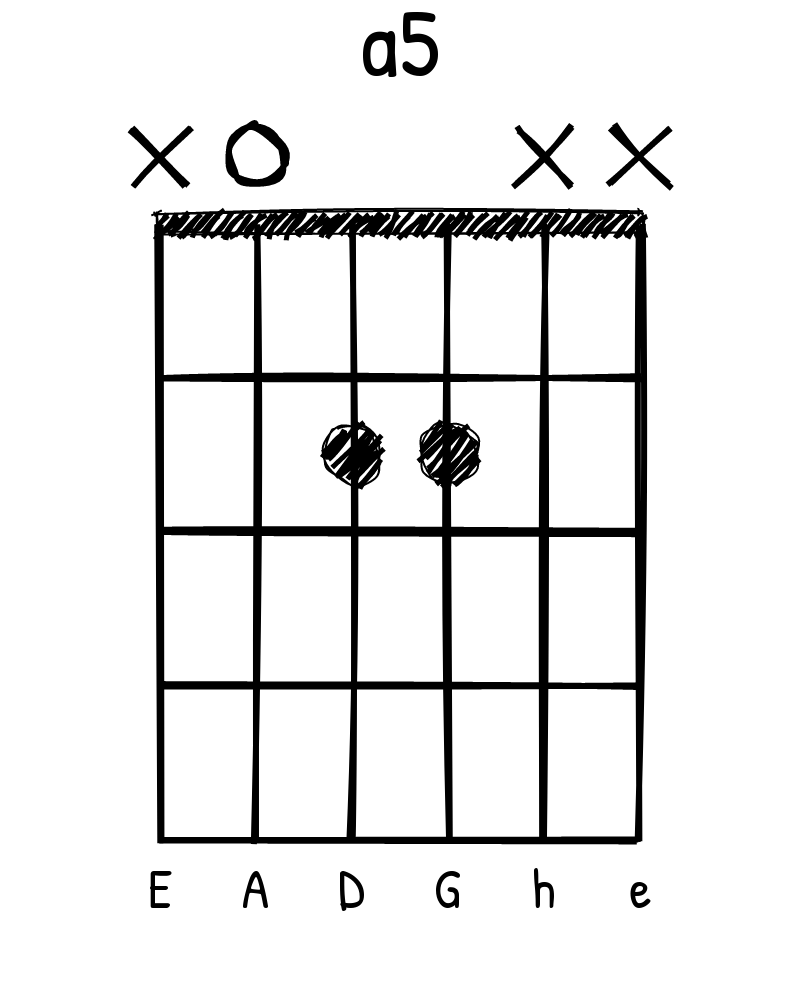
\includegraphics[height=3.5cm]{images/a5.png} \\
      \vspace{0.6cm}
      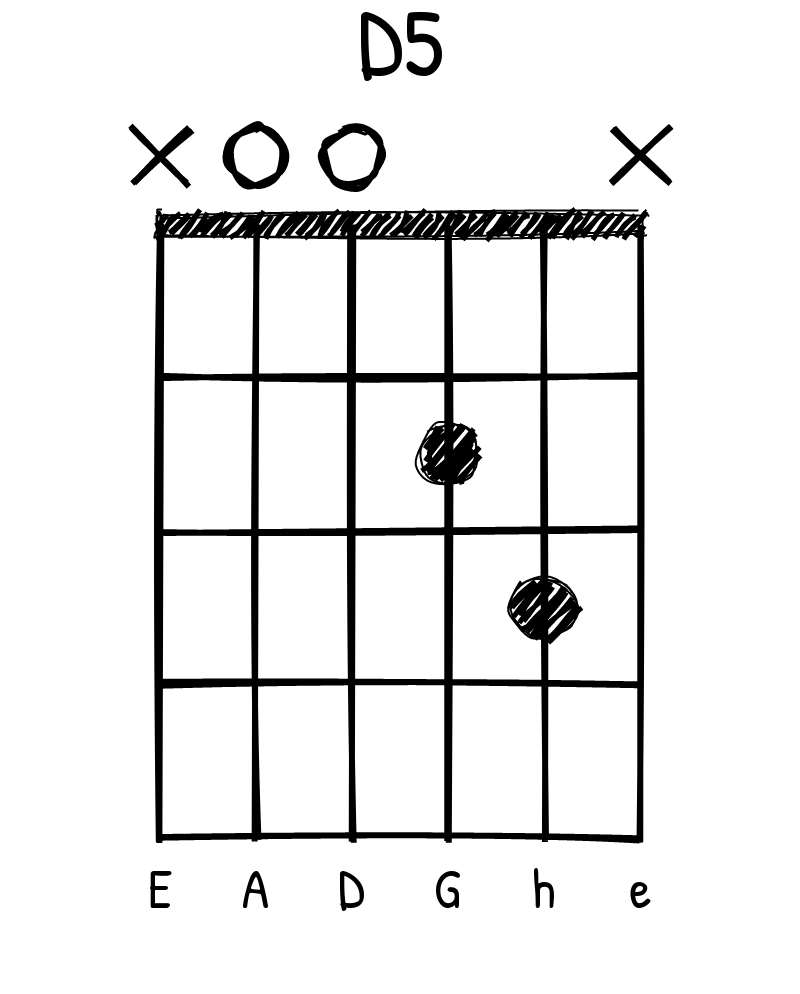
\includegraphics[height=3.5cm]{images/D5.png}
    \end{center}
    \end{multicols}
\end{song}


\newpage
\begin{song}{title={Premium Boy (Somebody That I Used To Know)}, music={Gotye}, interpret={808 Squad}}
\begin{multicols}{2}
    \small
    \begin{intro}
        \writechord{d} \writechord{C} \writechord{d} \writechord{C} $\times 4$
    \end{intro}
    \begin{verse}
        ^{d}Now and ^{C}then I think of ^{d}when we ^{C}were toge^{d}ther ^{C} ^{d} ^{C} \\
        ^{d} Like when you ^{C}said you felt so ^{d}happy ^{C}you could di^{d}e ^{C} ^{d} ^{C} \\
        ^{d} Told my^{C}self that you were ^{d}right for ^{C}me \\
        ^{d} But felt so ^{C}lonely in your ^{d}company ^{C} \\
        ^{d} But that was ^{C}love and it's an ^{d}ache I ^{C}still remem^{d}ber ^{C} ^{d} ^{C}
    \end{verse}
    \begin{interlude}
        \writechord{d} \writechord{C} \writechord{d} \writechord{C} $\times 4$
    \end{interlude}
    \begin{verse}
        You can get addicted to a certain kind of sadness \\
        Like resignation to the end, always the end \\
        So when we found that we could not make sense \\
        Well you said that we would still be friends \\
        But I'll admit that I was glad it was over
    \end{verse}
    \begin{chorus}
        ^{d} Bo ^{C}Michał to jest ^{B}premium ^{C}boy \\
        ^{d} Pije ^{C}kawę z mlekiem ^{B}sojowym gar^{C}dzi normal^{d}ną \\
        ^{C}Gardzi także ^*{B}herba ^{C}tą \\
        ^{d}Chyba że po^{C}słodzi cukrem ^*{B}trzcino ^{C}wym \\
        ^{d} Michał ^{C}to jest taki ^{B}premium ^{C}boy \\
        ^{d} Na jego ^{C}chlebie możesz ^{B}znaleźć tylko ^{C}  majo^{d}nez \\
        ^{C}Kiedyś zgłupiał ^{B}włączył ^{C}jazz \\
        ^{d}Potem wszedł na ^{C}łóżko i ze^{B}rzygał ^{C}się \\
        |: (bo Mi^{d}chał ^{C}--- to ^{B}premium bo^{C}y) | \\
        | ^{d}Każdy wie, że ^{C}Michał to jest ^{B}premium ^{C}boy :| \\
    \end{chorus}
    \begin{interlude}
        \writechord{d} \writechord{C} \writechord{d} \writechord{C} $\times 4$
    \end{interlude}
\end{multicols}
\end{song}


\newpage
\small
\begin{song}{title={Scenariusz dla moich sąsiadów}, music={Myslovitz}}
    \begin{intro}
        \writechord{A} \\
        \writechord{G} \writechord{F} \writechord{E}
    \end{intro}
    \begin{verse}
          ^{A} Kiedy powrócisz już ^{G} ja będę cz^{F}ekał ^{E} \\
        Ulicą pójdę wzdłuż kupię gazetę \\
        Zabiorę z sobą psa usiądę na ławce \\
        Skończę scenariusz by gotowy był \\
        Wieczorem
    \end{verse}
    \begin{chorus}
        ^{C}Wieczorem pr^{e}zed mym domem \\
        ^{F} Wystawię ekran i wyświetlę film ^{C} \\
        Coś o mnie i ^{e}o tobie \\
        ^{F} Będę leczył chore sąsiadów sny ^{C} ^{e}
    \end{chorus}
    \begin{interlude}
        \textit{akordy jak w zwrotce} \\
        oo oooo oo o o \\
        o oooo ooo ooo $\times 2$
    \end{interlude}
    \begin{verse}
        Z nieba przyleciał mój wielki przyjaciel \\
        Kiedy lądował ja jadłem kanapkę \\
        Wyśnił że chyba jest chorym człowiekiem \\
        Usiądź wygodnie i nie martw się \\
        Bo wieczorem
    \end{verse}
    \begin{chorus}
        Wieczorem przed mym domem\ldots
    \end{chorus}
    \begin{interlude}
        oo oooo oo o o \\
        o oooo ooo ooo $\times 2$
    \end{interlude}
    \begin{chorus} 
        Wieczorem przed mym domem\ldots $\times 2$
    \end{chorus}
\end{song}


\newpage
\begin{song}{title={Jest już za późno}, lyrics={Edward Stachura}, music={Stare Dobre Małżeństwo}}
    \begin{intro}
        \writechord{C} \writechord{F} \writechord{C} \writechord{F} 
    \end{intro}
    \begin{verse}
        ^{C}Jeszcze zdążymy w dżu^{d}ngli ludzkości ^{C}siebie odnaleźć ^{F} ^{C} \\
        ^{F} Tęskność zawr^{C}otna przybliża n^{d}as ^{G} \\
        ^{C}Zbiegną się wreszcie to^{d}ry sieroce n^{C}aszych dwóch planet ^{F} ^{C} \\
        ^{F} Cudnie spokr^{C}ewnią się ciała n^{d}am ^{G}
    \end{verse}    
    \begin{chorus}
        ^{e}Jest już za późno \\
        ^{F}Nie jest za późno \\
        ^{e}Jest już za późno \\
        ^{F}Nie jest za późno \\
        ^{e}Jest już za późno \\
        ^{F}Nie jest za ^{G}późno $\times 2$
    \end{chorus}
    \begin{verse}
        Jeszcze zdążymy tanio wynająć małą mansardę \\
        Z oknem na rzekę lub też na park \\
        Z łożem szerokim, piecem wysokim, ściennym zegarem \\
        Schodzić będziemy codziennie w świat 
    \end{verse}
    \begin{chorus}
        Jest już za późno\ldots $\times 2$
    \end{chorus}
    \begin{verse}
        Jeszcze zdążymy naszą miłością siebie zachwycić \\ 
        Siebie zachwycić i wszystko w krąg \\
        Wojna to będzie straszna, bo czas nas będzie chciał zniszczyć \\
        Lecz nam się uda zachwycić go
    \end{verse}
     \begin{chorus}
        Jest już za późno\ldots $\times 2$
    \end{chorus}
\end{song}


\newpage
\normalsize
\begin{song}{title={Space Oddity}, music={David Bowie}}
\begin{multicols}{2}
	\begin{intro}
	    \writechord{Fmaj7} \writechord{e} $\times 2$
	\end{intro}
    \begin{verse}    
        ^{C} Ground Control to Major To^{e}m \\
        ^{C} Ground Control to Major To^{e}m \\
        ^{a} Take your pro^{a/G}tein pills and \\
        P^{D/F#}ut your helmet on \\
        ^{C} Ground Control to Major To^{e}m \\
        \textit{(ten, nine, eight, seven, six)} \\
        ^{C} Commencing countdown, engines o^{e}n \\
        \textit{(five, four, three)}
         \\
        ^{a} Check igni^{a/G}tion and may \\
        ^{D/F#}God's love be with you \\
        \textit{(two, one, liftoff)} \\ \\
        \textit{6 taktów przerwy, \textbf{narastający chaos}} 
    \end{verse}
    \begin{verse}    
        ^{C}This is Ground Control to Major T^{E}om \\
        You've really made the gr^{F}ade \\
        And the pa^{f}pers want to kn^{C}ow whose shirts you w^{F}ear \\
        Now it's t^{f}ime to leave the cap^{C}sule if you d^{F}are \\
        Th^{C}sis is Major Tom to Ground Co^{E}ntrol \\
        I'm stepping through the do^{F}or \\
        And I'm fl^{f}oating in a m^{C}ost peculiar w^{F}ay \\
        And the st^{f}ars look very dif^{C}ferent tod^{F}ay 
    \end{verse}
    \begin{chorus}
        For he^{Fmaj7}re \\
        Am I si^{e}tting in a tin can \\
        ^{Fmaj7}Far above the wo^{e}rld \\
        ^{B}Planet Earth is b^{a}lue \\
        And there's n^{G}othing I can ^{F}do
    \end{chorus}
    \begin{interlude}
        |: C F G \\
        A A :|  \\
        \writechord{Fmaj7} e \\
        A C \\
        D E \\
    \end{interlude}
    \begin{verse}
        ^{C}Though I'm past one hundred thousand mi^{E}les \\
        I'm feeling very st^{F}ill \\
        And I th^{f}ink my spaceship kn^{C}ows which way to ^{F}go \\
        Tell my w^{f}ife I love her ve^{C}ry much she kn^{F}ows \\
    \end{verse}
    \begin{interlude}
        ^{G}Ground Control to ^{E7}Major Tom \\
        Your ^{a}circuit's dead, there's ^{a/G}something wrong \\
        Can you ^{D}hear me, Major Tom? \\
        Can you ^{C}hear me, Major Tom? \\
        Can you ^{G}hear me, Major Tom? \\
        Can you 
    \end{interlude}
    \begin{chorus}
        ^{Fmaj7}Here am I ^{e}floating 'round my tin can \\
        ^{Fmaj7}Far above the ^{e}moon \\
        ^{B}Planet Earth is ^{a}blue \\
        And there's ^{G}nothing I can ^{F}do
    \end{chorus}
\end{multicols}
\end{song}



% Ostatnia strona parzysta pusta, żeby nie było tekstu na odwrocie
\clearpage{\mbox{}\pagestyle{empty}\cleardoublepage}

\end{document}
